% Paquets généraux
\documentclass[a4paper,12pt,titlepage,twoside]{article}
\usepackage[T1]{fontenc}
\usepackage[utf8]{inputenc}
\usepackage[french]{babel}
\addto\captionsfrench{%
  \renewcommand{\tablename}{Tableau}%
}
\usepackage[gen]{eurosym}
%\usepackage[dvips]{graphicx}
\usepackage{fancyhdr}
\usepackage{pdfpages} 
\usepackage{multido}
\usepackage{hyperref}
%\usepackage{textcomp}
\usepackage{schemabloc}
\usepackage[bitstream-charter]{mathdesign}
\usepackage{array}
\newcolumntype{P}[1]{>{\centering\arraybackslash}p{#1}}

\newcommand{\id}{54}
\newcommand{\nom}{Liaisons mécaniques}
\newcommand{\sequence}{04}
\newcommand{\num}{01}
\newcommand{\type}{TP}
\newcommand{\descrip}{Modélisation d'un solide. Comportement des liaisons mécaniques. Modéliser les mécanismes du laboratoire par un schéma cinématique, paramétré.}
\newcommand{\competences}{A3-C4: Analyse d'architecture et de comportement \\ &  Mod1-C1: Isolement d'un solide ou d'un système de solides \\ &  Mod2-C10-1: Modèle de solide indéformable \\ &  Mod2-C11: Modélisation géométrique et cinématique des mouvements entre solides indéformables \\ &  Mod2-C12: Modélisation cinématique des liaisons entre solides \\ &  Mod2-C15: Modélisation des actions mécaniques \\ &  Rés-C6: Utilisation d'un solveur ou d'un logiciel multi physique \\ &  Com1-C1: Différents descripteurs introduits dans le programme \\ &  Com2-C4: Outils de communication}
\newcommand{\nbcomp}{9}
\newcommand{\systemes}{Plateforme Stewart}
\newcommand{\systemessansaccent}{Plateforme Stewart}
\newcommand{\ilot}{2}
\newcommand{\ilotstr}{02}
\newcommand{\dossierilot}{\detokenize{Ilot_02 Plateforme Stewart}}
\newcommand{\imageun}{Plateforme}

\newcommand{\urlsysteme}{\href{https://www.costadoat.fr/systeme/57}{Ressources système}}
\newcommand{\matlabsimscape}{\href{https://github.com/Costadoat/Sciences-Ingenieur/raw/master/Systemes/Plateforme Stewart/Plateforme_Stewart_Simscape.zip}{Modèle Simscape}}
\newcommand{\solidworks}{\href{https://github.com/Costadoat/Sciences-Ingenieur/raw/master/Systemes/Plateforme Stewart/Plateforme_Stewart_Solidworks.zip}{Modèle Solidworks}}
\newcommand{\edrawings}{\href{https://github.com/Costadoat/Sciences-Ingenieur/raw/master/Systemes/Plateforme Stewart/Plateforme_Stewart.EASM}{Modèle eDrawings}}
\newcommand{\test}{Stewart_param1}
\newcommand{\testi}{Stewart_param2}
\newcommand{\testii}{Stewart_param3}
\newcommand{\testiii}{Stewart_param4}
\newcommand{\testiiii}{Stewart_euler}

\newcommand{\institute}{Lycée Dorian}

\usepackage{fancyvrb}
\usepackage{color}
\usepackage{xcolor}
\usepackage{colortbl}
\usepackage{helvet}
\renewcommand{\familydefault}{\sfdefault}
\usepackage{amsfonts}
\usepackage{amsmath}
%\usepackage{xspace}
\usepackage{varioref}
\usepackage{tabularx}
%\usepackage{floatflt}
\usepackage{graphics}
\usepackage{wrapfig}
\usepackage{textcomp}
\usepackage{tikz}
\usepackage{wrapfig}
\usepackage{gensymb}
\usepackage[percent]{overpic}
\usepackage[european]{circuitikz}
\usetikzlibrary{babel}
\usepackage{ifthen}
\usepackage{cancel}
\usepackage{etoolbox}
\usepackage{multirow}
%\usepackage{boxedminipage}
\definecolor{gris25}{gray}{0.75}
\definecolor{bleu}{RGB}{18,33,98}
\definecolor{bleuf}{RGB}{42,94,171}
\definecolor{bleuc}{RGB}{231,239,247}
\definecolor{rougef}{RGB}{185,18,27}
\definecolor{rougec}{RGB}{255,188,204}%255,230,231
\definecolor{vertf}{RGB}{103,126,82}
\definecolor{vertc}{RGB}{220,255,191}
\definecolor{forestgreen}{rgb}{0.13,0.54,0.13}
\definecolor{blcr}{rgb}{0.59,0.69,0.84}
\definecolor{blfr}{rgb}{0.32,0.51,0.75}
\definecolor{orfr}{rgb}{0.90,0.42,0.15}
\definecolor{orcr}{rgb}{0.90,0.65,0.50}
\definecolor{orangef}{rgb}{0.659,0.269,0.072}
\definecolor{orange}{rgb}{0.58,0.35,0.063}
\definecolor{orangec}{rgb}{0.43,0.32,0.25}
\definecolor{rcorrect}{rgb}{0.6,0,0}
\definecolor{sequence}{rgb}{0.75,0.75,0.75}
\definecolor{competences}{rgb}{0.61,0.73,0.35}
\definecolor{grisf}{HTML}{222222}
\definecolor{grisc}{HTML}{636363}
\definecolor{normal}{HTML}{4087c4}
\definecolor{info}{HTML}{5bc0de}
\definecolor{success}{RGB}{92,184,92}
\definecolor{warning}{RGB}{240,173,78}
\definecolor{danger}{RGB}{217,83,79}
\hypersetup{                    % parametrage des hyperliens
    colorlinks=true,                % colorise les liens
    breaklinks=true,                % permet les retours à la ligne pour les liens trop longs
    urlcolor= blfr,                 % couleur des hyperliens
    linkcolor= orange,                % couleur des liens internes aux documents (index, figures, tableaux, equations,...)
    citecolor= forestgreen                % couleur des liens vers les references bibliographiques
    }

% Mise en page
\pagestyle{fancy}

\setlength{\hoffset}{-18pt}
\setlength{\oddsidemargin}{0pt} 	% Marge gauche sur pages impaire2s
\setlength{\evensidemargin}{0pt} 	% Marge gauche sur pages paires
\setlength{\marginparwidth}{00pt} 	% Largeur de note dans la marge
\setlength{\headwidth}{481pt} 	 	% Largeur de la zone de tête (17cm)
\setlength{\textwidth}{481pt} 	 	% Largeu\textbf{r de la zone de texte (17cm)
\setlength{\voffset}{-18pt} 		% Bon pour DOS
\setlength{\marginparsep}{7pt}	 	% Séparation de la marge
\setlength{\topmargin}{-30pt} 		% Pas de marge en haut
\setlength{\headheight}{55pt} 		% Haut de page
\setlength{\headsep}{20pt} 		% Entre le haut de page et le texte
\setlength{\footskip}{30pt} 		% Bas de\textbf{ page + séparation
\setlength{\textheight}{700pt} 		% Hauteur de l'icone zone de texte (25cm)
\setlength\fboxrule{1 pt}
\renewcommand{\baselinestretch}{1}
\setcounter{tocdepth}{1}
\newcommand{\cadre}[2]
{\fbox{
  \begin{minipage}{#1\linewidth}
   \begin{center}
    #2\\
   \end{center}
  \end{minipage}
 }
}

\newcommand{\repon}[1]
{
~\ \\
\begin{tabular}{|m{\linewidth}|}
 \hline
\multido{}{#1}{\\ \hline}
\end{tabular}
}

\newcounter{num_quest} \setcounter{num_quest}{0}
\newcounter{num_rep} \setcounter{num_rep}{0}
\newcounter{num_cor} \setcounter{num_cor}{0}

\newcommand{\question}[1]{\refstepcounter{num_quest}\par
~\ \\ \parbox[t][][t]{0.15\linewidth}{\textbf{Question \arabic{num_quest}}}\parbox[t][][t]{0.85\linewidth}{#1}\par
}


\newcommand{\reponse}[3]
{\refstepcounter{num_rep}
\noindent
\rule{\linewidth}{.5pt}\\
\textbf{Question \arabic{num_rep}:} ~\ \\
\ifdef{\public}{\multido{\i=1+1}{#1}{~\ \\}#2}{#3}
}

\newcommand{\cor}
{\refstepcounter{num_cor}
\noindent
\rule{\linewidth}{.5pt}
\textbf{Question \arabic{num_cor}:} \\
}

\newcommand{\repcarre}[2]
{
~\ \\
\begin{tikzpicture}
\draw [fill=white] (0,0) rectangle +(\linewidth,#1);
\node[align=left] at (1.1,#2-0.3) {\textbf{Question #1:}};
\end{tikzpicture}
}

\newcommand{\titre}[1]
{\begin{center}
\cadre{0.8}{\huge #1} 
\end{center}
}


% En tête et pied de page
\lhead{\nom}
\rhead{
\includegraphics[width=2cm]{../../img/logo}}
\lfoot{\auteurun,\ \auteurdeux}
\cfoot{Page \thepage}

\fancypagestyle{documentreponse}{%
  \fancyhf{}
  \fancyhead[LO]{Nom: ........................ Prénom: ........................}
  \fancyhead[LE]{\nom}
  \fancyhead[RE,RO]{
\includegraphics[width=2cm]{../../img/logo}}
  \lfoot{Document réponse}
  \cfoot{Page \thepage}
   }
  
\fancypagestyle{correction}{%
  \fancyhf{}
  \lhead{\colorbox{danger}{\begin{minipage}{0.65\paperwidth} \textcolor{white}{\textbf{Correction}} \end{minipage}} }
  \rhead{
\includegraphics[width=2cm]{../../img/logo}}
  \lfoot{Renaud Costadoat, Françoise Puig}
  \rfoot{\colorbox{danger}{\begin{minipage}{0.5\paperwidth} \begin{flushright}\textcolor{white}{\textbf{Correction}}\end{flushright} \end{minipage}} }}

\fancypagestyle{correctioninfo}{%
  \fancyhf{}
  \lhead{\colorbox{danger}{\begin{minipage}{0.65\paperwidth} \textcolor{white}{\textbf{Correction}} \end{minipage}} }
  \rhead{
\includegraphics[width=2cm]{../../img/logo}}
  \lfoot{Renaud Costadoat, Juliette Genzmer, Willie Robert}
  \rfoot{\colorbox{danger}{\begin{minipage}{0.6\paperwidth} \begin{flushright}\textcolor{white}{\textbf{Correction}}\end{flushright} \end{minipage}} }}

\renewcommand{\footrulewidth}{0.4pt}

\usepackage{eso-pic}
\newcommand{\BackgroundPic}{%
\put(0,0){%
\parbox[b][\paperheight]{\paperwidth}{%
\vfill
\begin{center}
\hspace{0.5cm}\vspace{0.5cm}
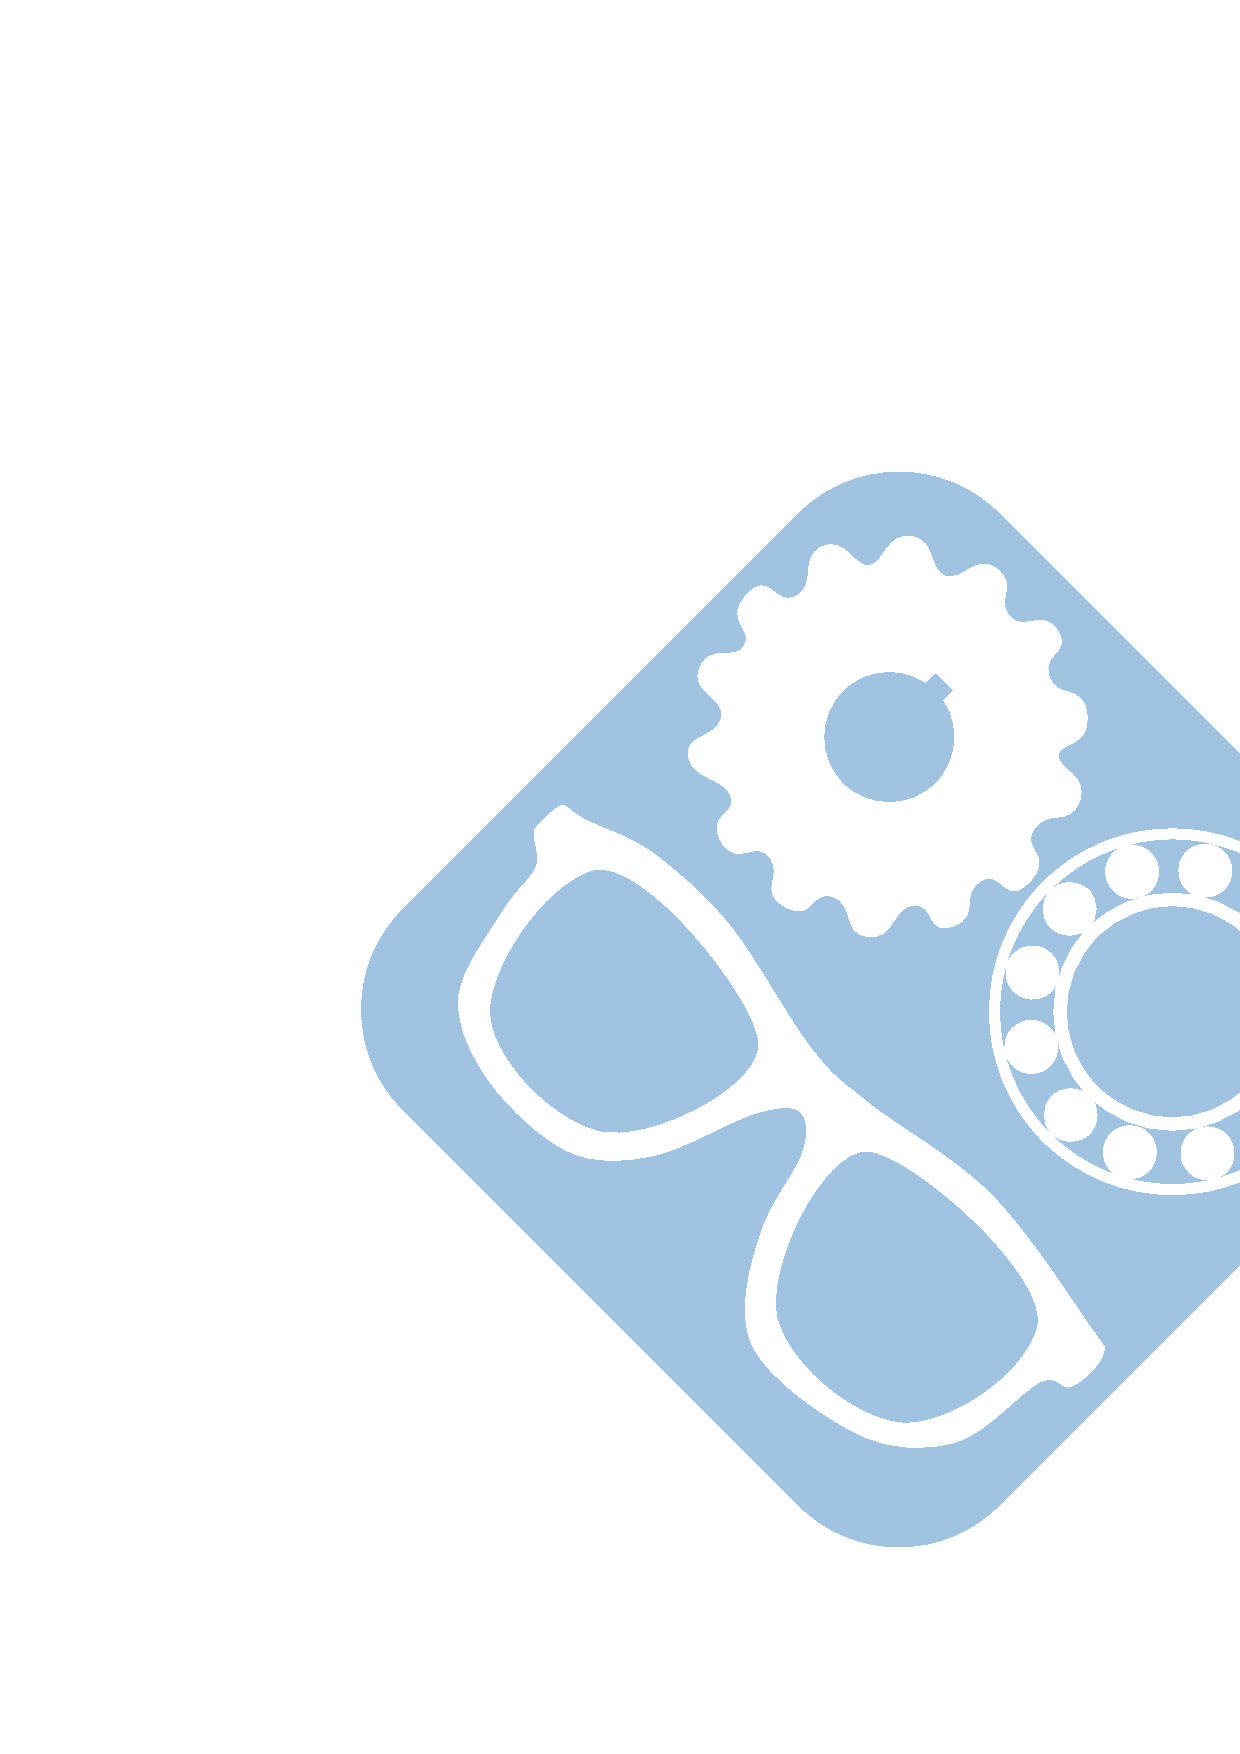
\includegraphics[width=\paperwidth,height=\paperheight,%
keepaspectratio]{../../img/fond3}%
\end{center}
\vfill
}}}

\newcommand{\BackgroundPicdeux}{%
\put(25,-30){%
\parbox[b][\paperheight]{\paperwidth}{%
\vfill
\begin{center}
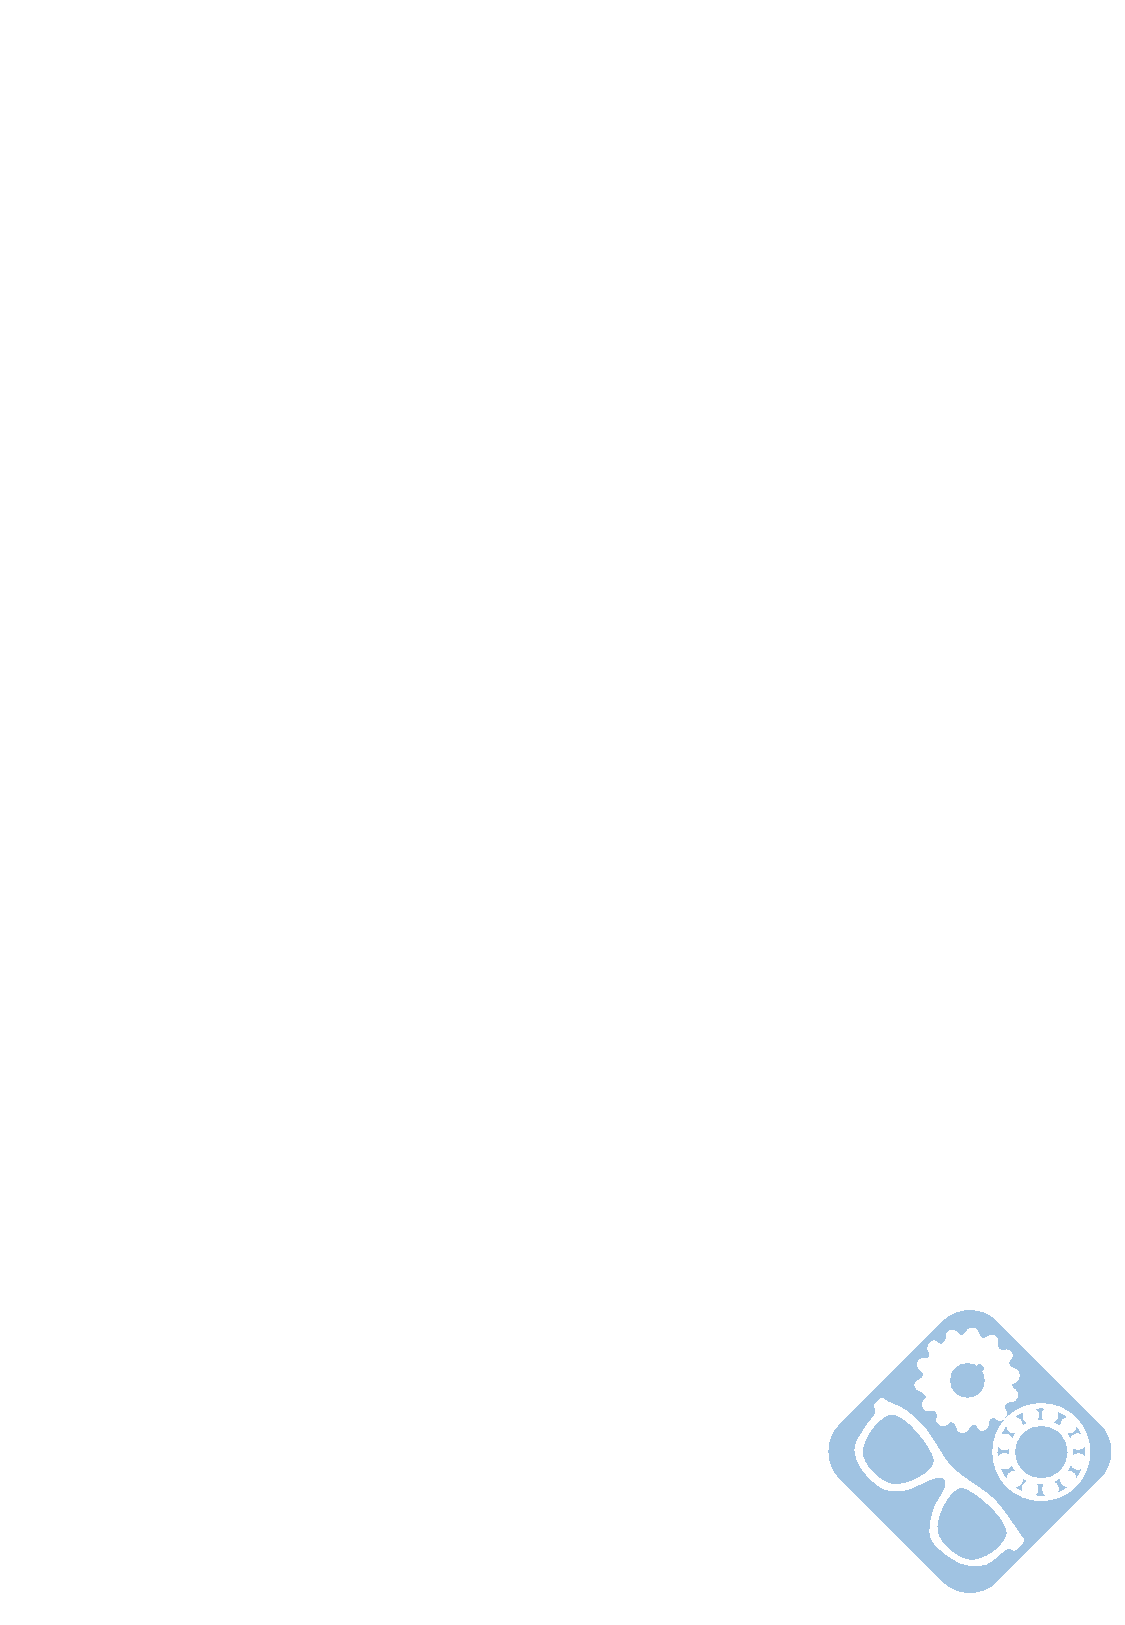
\includegraphics[width=\paperwidth,height=\paperheight,%
keepaspectratio]{../../img/fond4}%
\end{center}
\vfill
}}}

\begin{document}

\pagestyle{empty}

\AddToShipoutPicture*{\BackgroundPic}


\includegraphics[width=2cm]{../../img/logo}

\Huge{DS \num\ - \sujet}

\vspace{1cm}

\ifdef{\prive}{\begin{center}\colorbox{danger}{\Huge{Avec Correction}}\end{center}}{}

\begin{center}
\centering\huge{PTSI}
\end{center}

\vspace{2cm}


\begin{center}
\centering\Large{\jour}
\end{center}

\vspace{2cm}

\normalsize

\tableofcontents

\newpage

\AddToShipoutPicture{\BackgroundPicdeux}

\pagestyle{fancy}

\begin{center}
\Huge \sujet
\end{center}


\normalsize

\section{Dérailleurs de vélo de course Shimano Ultegra Di2}

\subsection{Présentation générale du système}

Le vélo fait partie des moyens de transport dont l'utilisation est en augmentation. En effet, depuis quelques années avec l'épuisement progressif des ressources fossiles (pétrole, charbon, gaz naturel,...), les ingénieurs cherchent à diversifier les moyens de transport. Le vélo revient ainsi sur le devant de la scène.

Différents types de vélos existent sur le marché permettant de répondre à des besoins spécifiques que l'on pourrait classer suivant plusieurs catégories :

\begin{center}
\begin{tabular}{|c|c|c|}
\hline
Type d'utilisation	& Lieu d'utilisation & Assistance\\
\hline
utilisation en loisir, & en ville, & Avec ou sans \\
utilisation sportive, & sur route, & \\
utilisation en compétition. & sur des chemins, & \\
& en montagne,... & \\
\hline
\end{tabular}
\end{center}

Dans ce sujet, nous étudierons le système de changement de vitesses sur un vélo de route conçu pour une utilisation en compétition avec dérailleurs électriques (et bien sûr sans utilisation d'assistance à la propulsion du vélo).

Le dérailleur est un système qui permet de changer le rapport de réduction entre la vitesse de rotation du pédalier et la vitesse de rotation des roues. Il se place sur la chaîne du vélo et déplace la chaîne pour la placer au niveau d'un plateau (dérailleur avant) et au niveau d'un pignon (dérailleur arrière). Une action du cycliste sur la commande séquentielle du dérailleur au niveau des manettes permet de « monter » ou de « descendre » le rapport vitesse et ainsi d'adapter l'action à fournir par le cycliste selon sa volonté.

La société Shimano conçoit des dérailleurs pour tous types de vélos. Nous nous intéresserons au dérailleur Shimano Ultegra Di2 Série 6870.

\begin{figure}[!h]
 \centering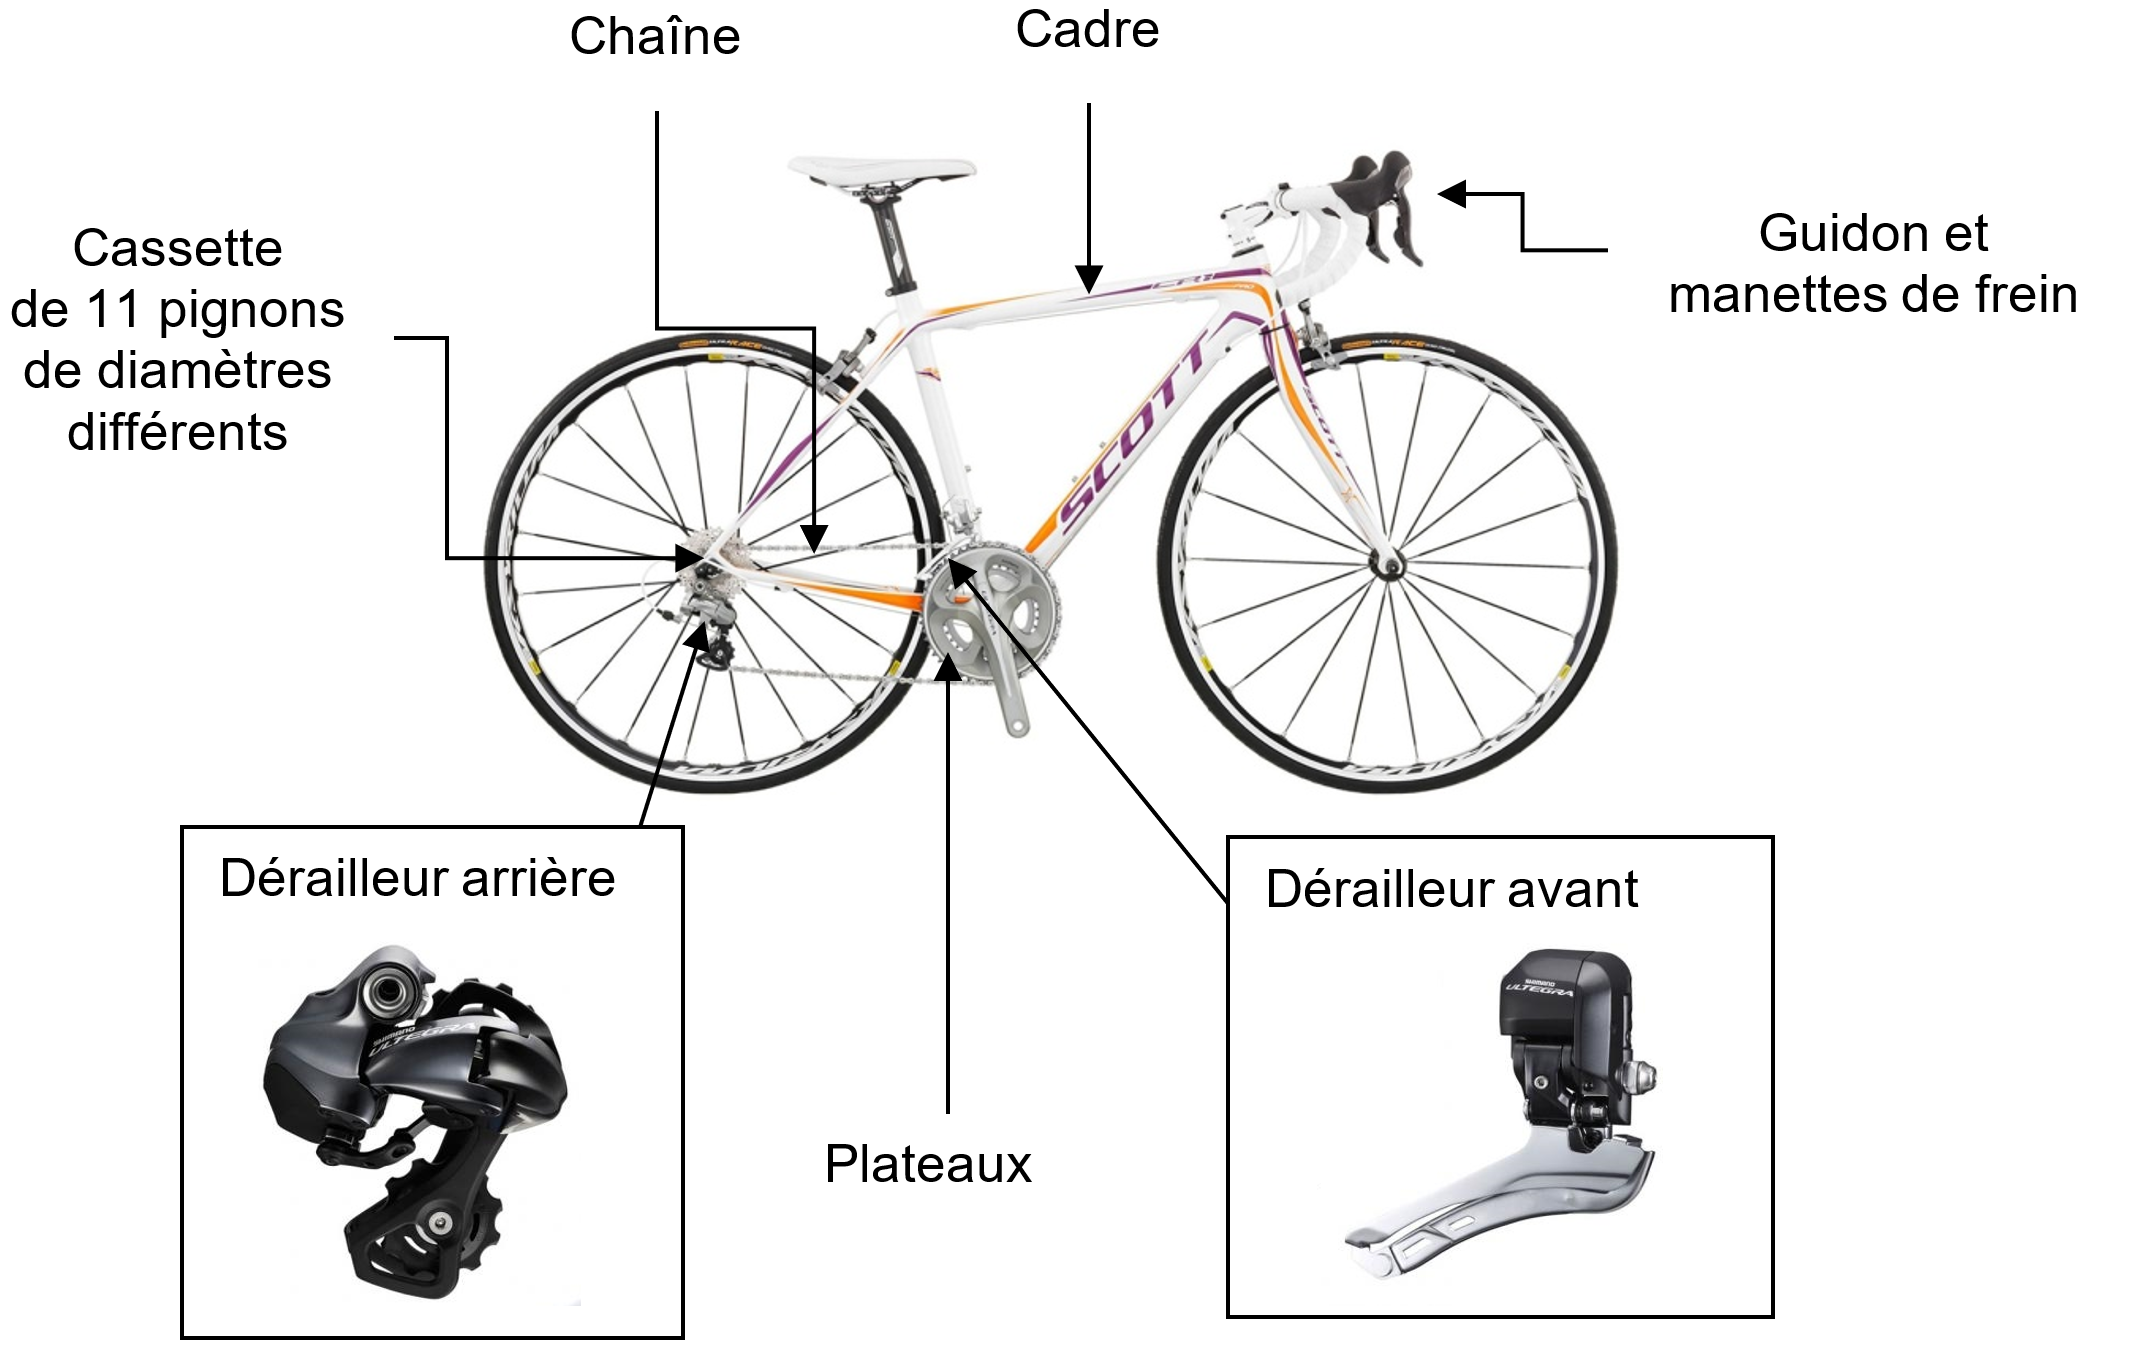
\includegraphics[width=0.7\linewidth]{img/img01}
 \caption{Vélo de course}
 \label{img01}
\end{figure}

\begin{figure}[!h]
 \centering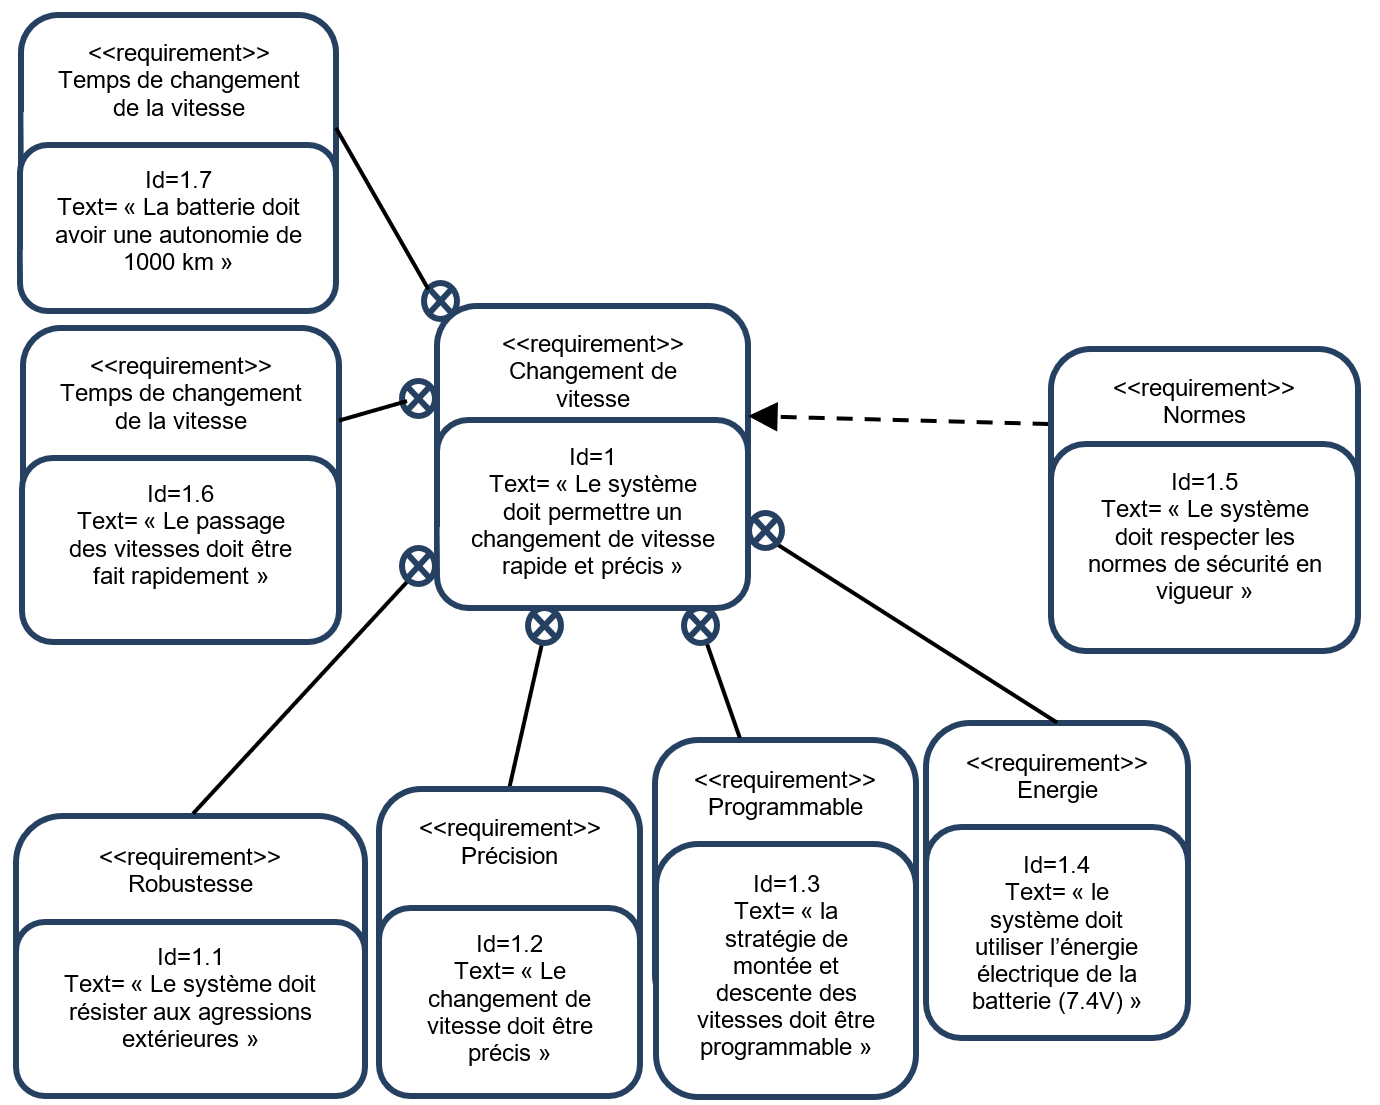
\includegraphics[width=0.8\linewidth]{img/img02}
 \caption{Diagramme des exigences du dérailleur arrière}
 \label{img02}
\end{figure}

\newpage

Extrait du cahier des charges :
\begin{center}
\begin{tabular}{|c|c|c|}
\hline
Exigence & Critères & Niveaux \\
\hline
1.2	& Précision par rapport à la position centrée & 0,34 mm \\
\hline
1.2	& Distance entre le galet de guidage et les pignons & non contact \\
\hline
1.3	& Adaptation au type de parcours & Route, cyclocross, VTT \\
\hline
1.6	& Temps de changement de vitesse (valeur en s) & < 0,3 s \\
\hline
1.6	& Dépassement (valeur en mm) & = 0,5 mm \\
\hline
1.7 & Autonomie de la batterie & 1000 km \\
\hline
\end{tabular}
\end{center}

~\ \\
L'exigence de rapidité 1.6 est associée de manière évidente à un critère temporel mais elle nécessite également de cibler un dépassement de 0,5 mm afin que la chaîne puisse « accrocher» plus rapidement le pignon demandé. Au-delà de cette valeur, on pourrait engager le pignon suivant et en dessous de cette valeur, le passage serait moins rapide. 

\subsection{Validation de la géométrie choisie pour les changements de vitesses à l'arrière.}

\textit{Objectif : Vérifier que le dérailleur arrière du vélo permette de positionner la chaîne en face du pignon désiré par le cycliste.}

\textbf{Choix de la loi d'évolution du déplacement de la chape de dérailleur}

Le dérailleur arrière Shimano se fixe sur le cadre du vélo, proche de l'axe de la roue arrière.

\begin{figure}[!h]
 \centering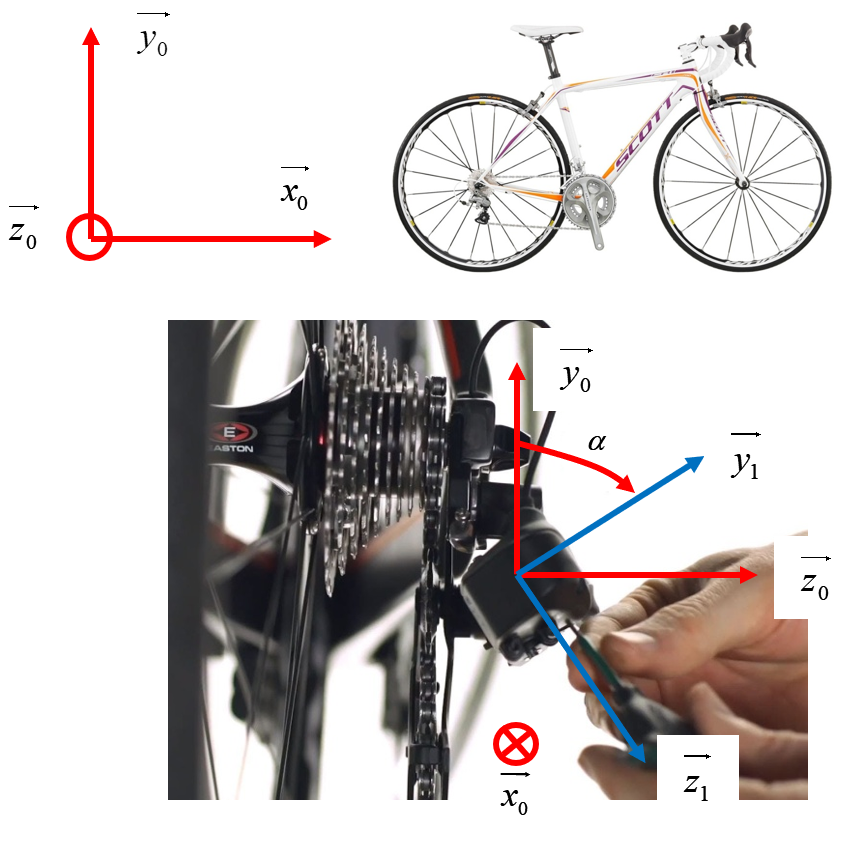
\includegraphics[width=0.5\linewidth]{img/img03}
 \caption{Vélo vu de l'arrière}
 \label{img03}
\end{figure}

L'angle $\alpha=(\overrightarrow{y_0},\overrightarrow{y_1})=(\overrightarrow{z_0},\overrightarrow{z_1})$ est fixe et vaut : $\alpha=50\degree$.

D'un point de vue cinématique, le dérailleur peut se modéliser par un parallélogramme articulé (appelé « système 4 barres ») dans le plan $(\overrightarrow{x_1},\overrightarrow{y_1})$. En effet, comme l'illustre le modèle ci-après, le parallélogramme ABCD se déforme.

\subsubsection{Modèle simplifié (modèle plan)}

\begin{figure}[!h]
 \centering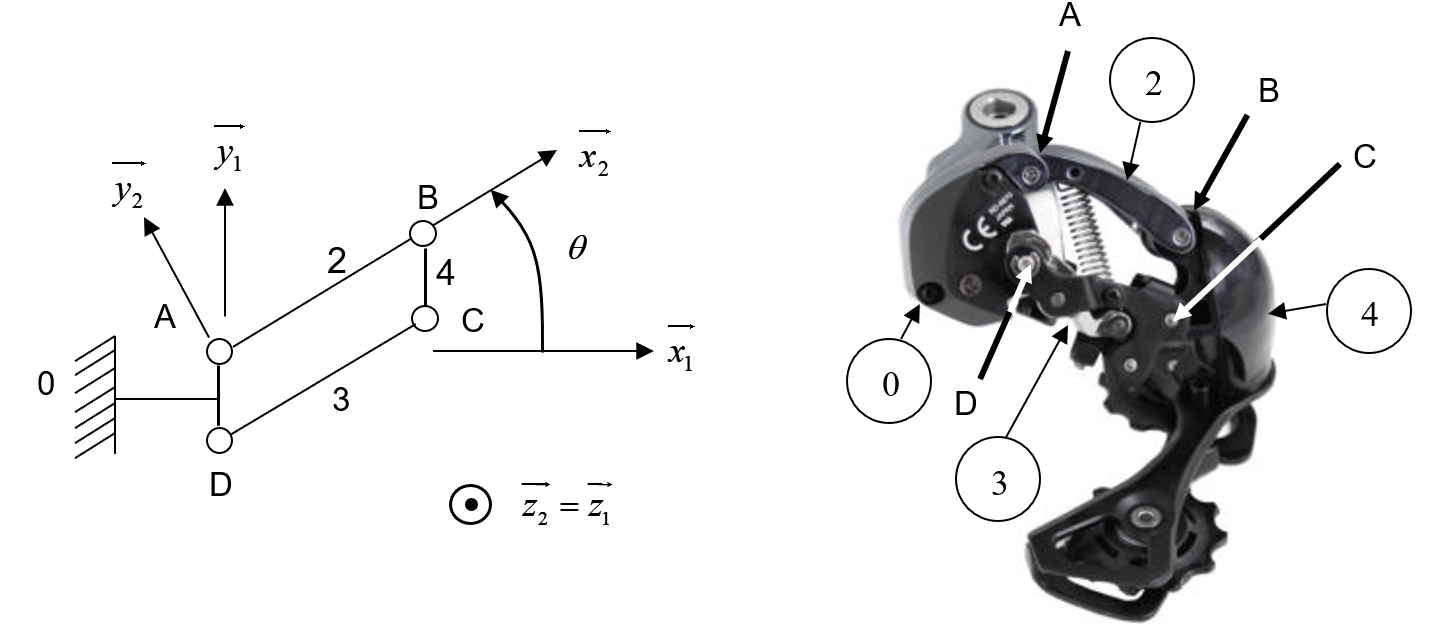
\includegraphics[width=0.8\linewidth]{img/img04}
 \caption{Modélisation du dérailleur dans le plan $(\protect\overrightarrow{x_1},\protect\overrightarrow{y_1})$}
 \label{img04}
\end{figure}

\begin{itemize}
 \item 0: Cadre du vélo (supposé fixe),
 \item 2 et 3: Biellettes intermédiaires,
 \item 4: Chape de dérailleur.
\end{itemize}

Paramétrage :\\
$\left\{\begin{array}{l}
\overrightarrow{AB}=\overrightarrow{DC}=L.\overrightarrow{x_2} \\
\overrightarrow{DA}=\overrightarrow{CB}=l.\overrightarrow{y_1}
\end{array}\right.$  avec 
$\left\{\begin{array}{l}
L=30mm \\
l=13mm
\end{array}\right.$ 

L'axe $(A,\overrightarrow{z_1})$ passe par le point O' (voir annexe A).

On note $\theta$ l'angle qui positionne l'axe $(A,\overrightarrow{x_2})$ par rapport à l'axe $(A,\overrightarrow{x_1})$. Il varie entre -60° et 60°.

Le fabricant a choisi un système 4 barres réalisé avec 4 liaisons pivots pour permettre le changement de vitesses. Ceci permet à la chape de dérailleur d'avoir un mouvement de translation par rapport au cadre du vélo et donc de ne pas tordre la chaîne.

\question{Faire le graphe de liaison \textbf{complet} du mécanisme.}

\question{Tracer les figures de changement de base permettant d'écrire la base $B_2(\overrightarrow{x_2},\overrightarrow{y_2},\overrightarrow{z_2})$ dans la base $B_1(\overrightarrow{x_1},\overrightarrow{y_1},\overrightarrow{z_1})$ et $B_1(\overrightarrow{x_1},\overrightarrow{y_1},\overrightarrow{z_1})$ dans la base $B_0(\overrightarrow{x_0},\overrightarrow{y_0},\overrightarrow{z_0})$ on prendra:
\begin{itemize}
\item $0<\theta<\frac{\pi}{2}$,
\item $0<\alpha<\frac{\pi}{2}$,
\item $\overrightarrow{x_0}$ perpendiculaire à la feuille dirigé vers le lecteur,
\item $\overrightarrow{y_0}$ vers la droite,
\item $\overrightarrow{z_1}$ perpendiculaire à la feuille dirigé vers le lecteur,
\item $\overrightarrow{x_1}$ vers la droite.
\end{itemize}}

\question{Déterminer la fermeture géométrique issue de la figure \ref{img04}. Celle-ci nous permettra d'obtenir la position de la barre (BC) en fonction de $\theta$.}

\question{Déterminer les torseurs des 4 liaisons de la figure \ref{img04}.}

On utilisera le formalisme suivant pour décrire le torseur cinématique de la liaison entre les pièces $i$ et $j$ au point $M$ dans la base $B$:
\begin{center}
$\left\{V_{i/j}\right\}=\left\{\begin{array}{cc}\omega_{xij} & V_{M,xij} \\ \omega_{yij} & V_{M,yij} \\ \omega_{zij} & V_{M,zij} \end{array}\right\}_{M,B}$
\end{center}

\question{Déplacer ces torseurs au point A dans la base $B_1$.}

On donne la fermeture cinématique suivante:

$\left\{V_{4/2}\right\}+\left\{V_{2/0}\right\}=\left\{V_{4/3}\right\}+\left\{V_{3/0}\right\}$

\question{Écrire les 6 équations scalaires qui en résultent, en projection dans la base $B_1$.}

\question{En déduire la valeur numérique de $\|\overrightarrow{\Omega_{4/0}}\|$ et en déduire l'orientation de la droite (BC) en fonction de $\theta$.}

~\

Soit:\\
\begin{itemize}
 \item $B_1$ la position de $B$ la plus basse,
 \item $B_2$ la position de $B$ la plus haute.
\end{itemize}

\question{Exprimer le vecteur position $\overrightarrow{AB}$ dans la base $(\overrightarrow{x_1},\overrightarrow{y_1},\overrightarrow{z_1})$ en fonction de l'angle $\theta$.}

\question{Déterminer le vecteur $\overrightarrow{B_1B_2}$ dans la base $B_1$.}

\question{En déduire l'expression du déplacement $d=\overrightarrow{AB}.\overrightarrow{z_0}$ de la chape de dérailleur projeté suivant l'axe $(A,\overrightarrow{z_0})$.}

%Pour une cassette de 11 pignons, le fabricant préconise de régler à la main l'alignement de la chape de dérailleur avec le pignon central (le 6ème, le plus grand sera noté le 1er pignon). Ensuite on place la chape de dérailleur (voir annexe A) dans chacune des deux positions extrêmes (en face du petit pignon puis du grand pignon) afin de régler les deux butées de fin de course. 
%
%\question{Justifier pourquoi le fabricant fait la préconisation de se caler sur le 6\up{ème} pignon.}

~\

On suppose que pour passer d'un pignon au pignon voisin, le système de commande du dérailleur électrique Di2 fait tourner le moteur (voir annexes A et C) du même angle à chaque fois. Comme l'illustre l'annexe B, la largeur intérieure de la chaîne, dimension laissant passer l'épaisseur d'un pignon, est de 2,18 mm. Un pignon mesure 1,5 mm d'épaisseur. La distance entre 2 pignons consécutifs est de 4 mm. 

\question{D'après les dimensions données, donner la valeur du défaut de positionnement suivant $\overrightarrow{z_0}$
par rapport à la position centrée que l'on peut accepter pour que la chaîne puisse s'accoupler au pignon choisi.}

~\

On fournit sur le document réponse l'évolution de la distance $d$ en fonction de l'angle $\theta$ trouvée à la question 10.

\question{Approximer graphiquement par une droite l'évolution proposée sur le document réponse en minimisant l'erreur maximale. }

\question{Estimer sur le graphique l'erreur de positionnement maximale faite entre la loi calculée et la loi linéaire. Est-ce acceptable avec les valeurs de largeurs de chaîne et de pignon données ? Conclure.}

~\

%Éviter le contact entre les pignons arrières et le galet de guidage (exigence 1.2).

%L'annexe D permet de visualiser le galet de guidage. Le fabricant propose différents étagements de pignons arrières (cassettes) selon les parcours empruntés par le cycliste, et son niveau sportif. Les valeurs données dans le tableau ci-dessous correspondent aux nombres de dents de chaque pignon pour deux cassettes différentes.
%
%Cassettes Shimano Ultegra CS-6800 11 vitesses :
%\begin{center}
%\begin{tabular}{|c|c|c|c|c|c|c|c|c|c|c|c|c|}
%\hline
% & Nom & \multicolumn{11}{c|}{Nombres de dents}\\
%\hline
%Cassette 1 & 11-23 & 11 & 12 & 13 & 14 & 15 & 16 & 17 & 18 & 19 & 21 & 23 \\
%\hline
%Cassette 2 & 11-32 & 11 & 12 & 13 & 14 & 15 & 17 & 19 & 21 & 23 & 25 & 28 \\
%\hline
%\end{tabular}
%\end{center}
%
%Par analogie avec les engrenages, on considère qu'une roue dentée se comporte cinématiquement comme un cylindre de diamètre $D_1$. La relation entre le diamètre $D_1$ et le nombre de dents $Z_i$ de chaque pignon $i$ est donc : $D_i=m.Z_i$ avec $m$ le module de l'engrènement $(m=3,3mm)$.
%
%Pour le réglage du jeu entre le dérailleur et les pignons dans le plan $(\overrightarrow{x_0},\overrightarrow{y_0})$, le fabricant préconise de placer le dérailleur arrière à $a=5mm$ du plus grand pignon arrière.
%
%\begin{center}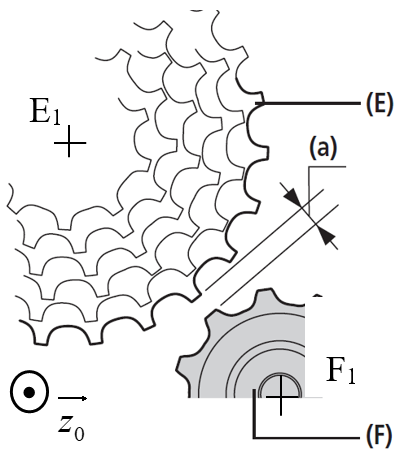
\includegraphics[width=0.4\linewidth]{img/img05}\end{center}
%
%\begin{itemize}
% \item (E) est le grand pignon arrière de centre $E_1$,
% \item (F) est le galet de guidage de centre $F_1$ tenu par la chape de dérailleur.
%\end{itemize}
%
%~\

%L'expression du déplacement d de la chape de dérailleur suivant $\overrightarrow{z_0}$ est :  $d=L.sin \theta.sin \alpha$ 
%
%On suppose que le déplacement du centre $F_1$ du galet de guidage (F) s'effectue dans le plan défini par les deux vecteurs : $(\overrightarrow{E_1F_1},\overrightarrow{z_0})$. Le point $E_1$ est supposé fixe.
%
%\question{Pour les dimensions de la cassette données dans l'annexe B, déterminer quelle est la valeur minimale de l'angle $\alpha$ pour pouvoir déplacer la chape de dérailleur sur toute l'épaisseur de la cassette. Comparer avec la valeur choisie par le fabricant $(\alpha=50\degree)$ et conclure sur la possibilité de changement de vitesse.}

%On cherchera à assurer que le galet de guidage reste toujours à peu près à la même distance des pignons.
%
%\question{En utilisant le tableau et le schéma proposés dans le document réponses, donner une estimation de l'angle $\alpha_{moyen}$ que l'on doit avoir pour suivre « au mieux » les pignons des différentes cassettes arrières données en se basant sur les diamètres mini et maxi de chaque cassette. Comparer avec l'angle $\alpha$ trouvé à la question précédente.}
%
%\question{On règle le galet de guidage à $a=5mm$ du plus grand pignon comme le préconise le fabricant. L'angle $\alpha$ vaut toujours 50°. En utilisant le schéma proposé dans le document réponses, déterminer à quelle distance e se trouvera le galet de guidage du petit pignon dans l'autre cas extrême pour chaque cassette. Commenter les résultats.}
%

En réalité, le déplacement du centre du galet de guidage (F) ne s'effectue pas dans le plan $(\overrightarrow{E_1F_1},\overrightarrow{z_0})$. Le calcul devient donc plus compliqué. Nous allons utiliser un modèle numérique (tridimensionnel) pour avoir des résultats plus pertinents et plus proches de la réalité.

\subsubsection{Modèle numérique (tridimensionnel)}

On rappelle que le point O est défini comme étant au centre de la cassette (centre du 6\up{ème} pignon). Les coordonnées (données en mm) du vecteur $\overrightarrow{OF_1}=X_{F_1}.\overrightarrow{x_0}+Y_{F_1}.\overrightarrow{y_0}+Z_{F_1}.\overrightarrow{z_0}$
dans le repère $(O,\overrightarrow{x_0},\overrightarrow{y_0},\overrightarrow{z_0})$ sont représentées ci-après :

\begin{figure}[!h]
 \centering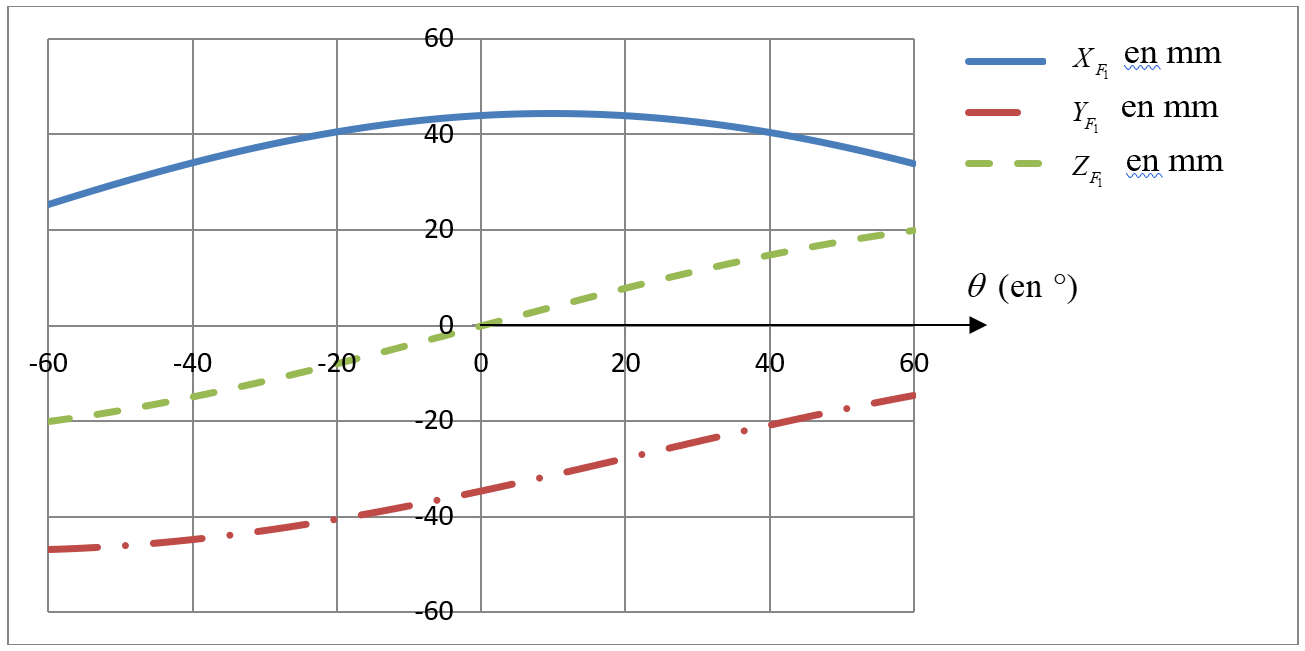
\includegraphics[width=0.8\linewidth]{img/img06}
 \caption{Coordonnées du vecteur $\protect\overrightarrow{OF_1}$ en mm dans le repère $(\protect\overrightarrow{x_0},\protect\overrightarrow{y_0},\protect\overrightarrow{z_0})$ en fonction de $\theta$ en °}
 \label{img06}
\end{figure}

La distance $e(Z_{F_1})$ entre le galet de guidage et la cassette sont représentés ci-après :

\begin{figure}[!h]
 \centering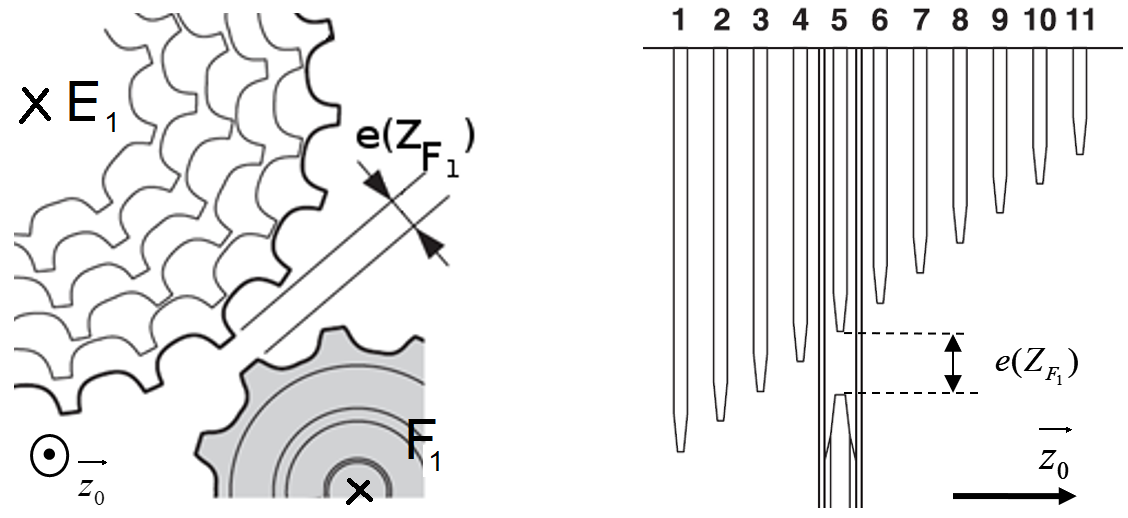
\includegraphics[width=0.8\linewidth]{img/img07}
 \caption{Distance $e(Z_{F_1})$}
 \label{img07}
\end{figure}

\begin{figure}[!h]
 \centering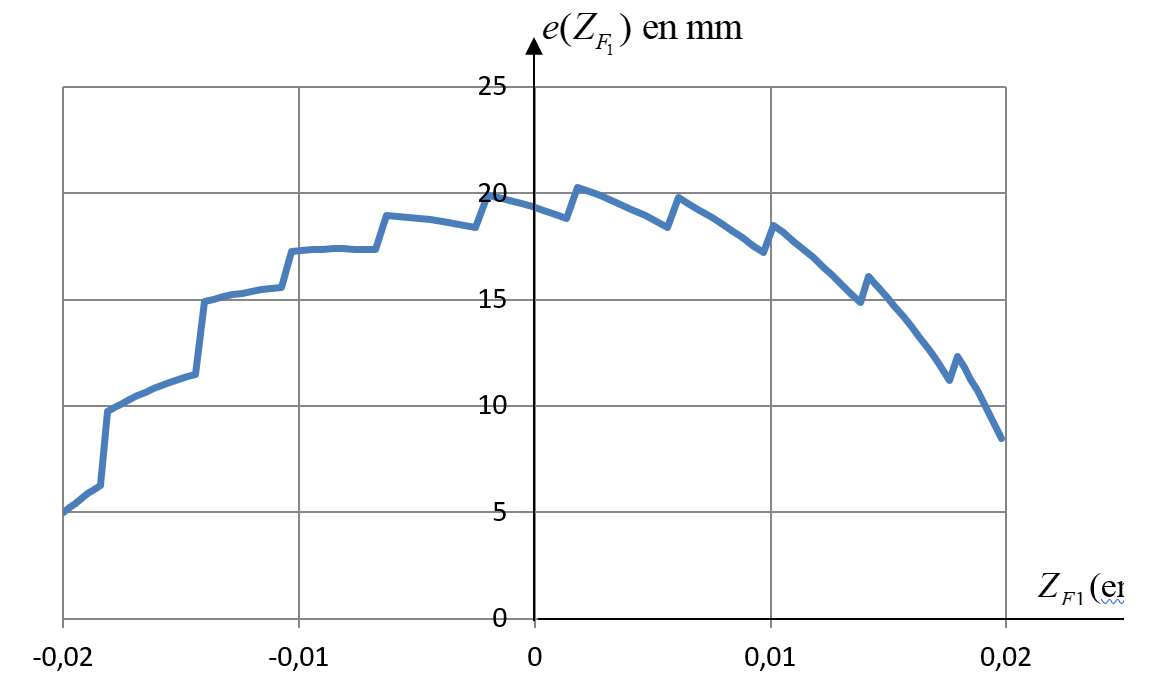
\includegraphics[width=0.8\linewidth]{img/img08}
 \caption{Distance $e(Z_{F_1})$ en mm du galet de guidage à la cassette en fonction de la position $Z_{F_1}$ de la chape sur l'axe $(O,\protect\overrightarrow{z_0})$.}
 \label{img08}
\end{figure}

On note $R_{galet}$ le rayon de tête du galet de guidage (F) et $R_{pignon}(Z_{F_1})$ le rayon de tête du pignon situé à la position $Z_{F_1}$ sur l'axe $(O,\overrightarrow{z_0})$.

\question{Exprimer la distance du galet de guidage aux pignons $e(Z_{F_1})$ en fonction de $X_{F_1}$, $Y_{F_1}$, $R_{galet}$ et $R_{pignon}(Z_{F_1})$. Expliquer d'où vient la forme en escalier de la courbe obtenue.}

\question{D'après la simulation numérique, le dérailleur permet-il de changer les 11 vitesses sans que les pièces ne se touchent (exigence1.2) ? Justifier.}

\question{Justifier le réglage du jeu de 5 mm entre le galet de guidage et le grand pignon préconisé par le fabricant. Expliquer pourquoi il n'a pas choisi de régler ce jeu avec le pignon médian, ou avec le petit pignon.}

\subsection{Validation du temps de changement de vitesse}

\textit{Objectif : Valider les critères associés à l'exigence 1.6 de rapidité de changement de vitesse.}

Le dérailleur arrière est composé d'un moteur à courant continu accouplé à un réducteur (voir annexe C). Le moteur est alimenté par une batterie Li-Ion :
\begin{itemize}
 \item Tension nominale 7.4 V,
 \item Capacité nominale 530 mAh.
\end{itemize}

Le schéma bloc du dérailleur arrière est représenté ci-dessous :
\begin{figure}[!h]
 \centering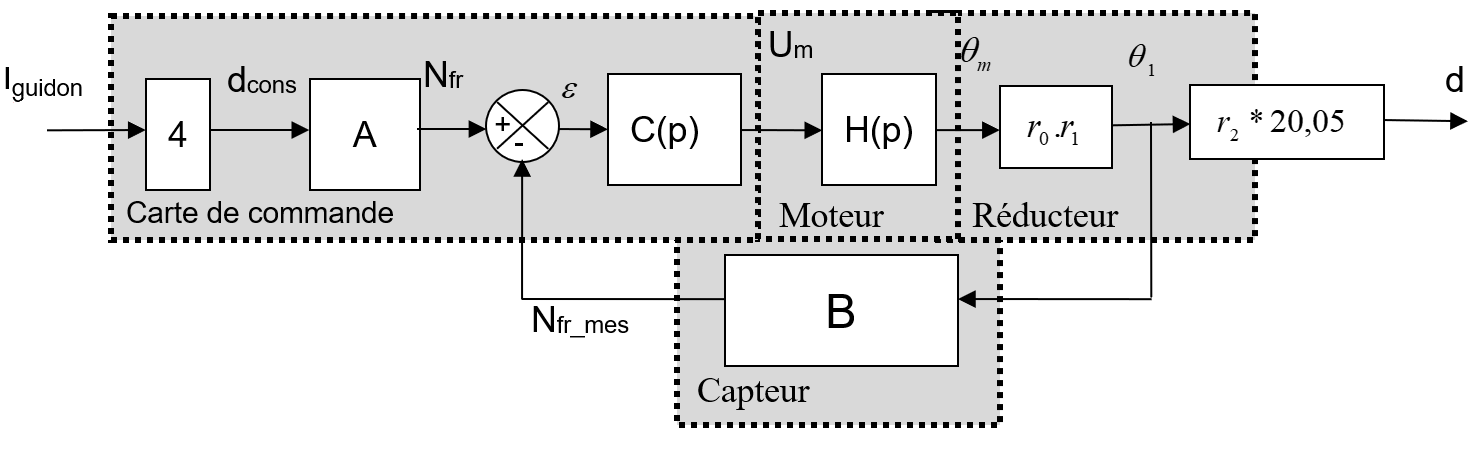
\includegraphics[width=0.8\linewidth]{img/img09}
 \caption{Schéma bloc du dérailleur arrière}
 \label{img09}
\end{figure}

Variables utilisées :
\begin{itemize}
 \item $I_{guidon}$: nombre d'impulsions données au guidon (sans unité),
 \item $d_{cons}$: déplacement de consigne du dérailleur arrière (en mm),
 \item $N_{fr\_mes}$: nombre de fronts (montants et descendants) mesurés sur le codeur,
 \item $\theta_{m}$: angle de rotation du moteur en radian,
 \item $\theta_1$: angle de rotation de l'arbre de sortie du réducteur en radian.

\end{itemize}

Rapports de transmission :
\begin{itemize}
 \item Roue vis sans fin : $r_0=\frac{\theta_{RV}}{\theta_{m}}$,
 \item Réducteur 1 : $r_1=\frac{\theta_{1}}{\theta_{RV}}$,
 \item Réducteur 2 : $r_2=\frac{\theta}{\theta_{1}}$,
\end{itemize}

Valeurs numériques :
\begin{itemize}
 \item $r_0r_1r_2=\frac{1}{1000}$,
 \item $r_2=\frac{1}{50}$.
\end{itemize}
 
On supposera que le nombre d'impulsions données au guidon correspond au nombre de pignons à passer sur le dérailleur arrière.

Le codeur incrémental comporte $n=7$ fentes et 2 voies et permet donc de détecter 28 positions par tour. Il sera considéré comme un système linéaire dans cette étude.

%La fonction de transfert $H(p)$ du moteur à courant continu est :
%\begin{center}
%$H(p)=\frac{K}{p.\left(K^2+J.p.\left(R+L.p\right)\right)}$
%\end{center}

Données:
\begin{itemize}
 \item $R=3,6\Omega$,
 \item $K=5,6mNm.A^{-1}=0,0056rad.s^{-1}.V$,
 \item $J=7,1.10^{-9}kg.m^2$,
 \item $L=0,05mH$.
\end{itemize}

En régime nominal, le moteur tourne à $15000tr.min^{-1}$.

\question{Montrer que $H(p)=\frac{K}{p.\left(K^2+J.p.\left(R+L.p\right)\right)}$.}

\question{Justifier le bloc avec le gain pur de \og 4 \fg. En déduire l'unité du \og 4 \fg et de $d_{cons}$.}

\question{Déterminer la relation entre $\theta_1$ et $N_{fr\_mes}$ puis l'expression analytique du gain $B$ et son unité.}

Pour la suite, on prendra $B=4,4$.

\question{Déterminer l'expression analytique du gain $A$ en fonction de $B$ et de $r_2$ à mettre dans le schéma bloc pour que $\epsilon$ soit nul lorsque $d=d_{cons}$, faire l'application numérique.}

~\

On suppose que le correcteur est proportionnel : $C(p)=K_{cor}$. 

On prend $K_{cor}$ égal à 1 pour l'instant.

\question{Calculer la fonction de transfert en boucle fermée $H_{BF}=\frac{d}{I_{guidon}}$ et la proposer sous forme canonique.}

~\

On donne ci-dessous l'allure de la réponse indicielle de la fonction de transfert du troisième ordre obtenue précédemment et de la réponse indicielle lorsqu'on néglige le terme d'ordre trois de cette fonction.

\begin{figure}[!h]
 \centering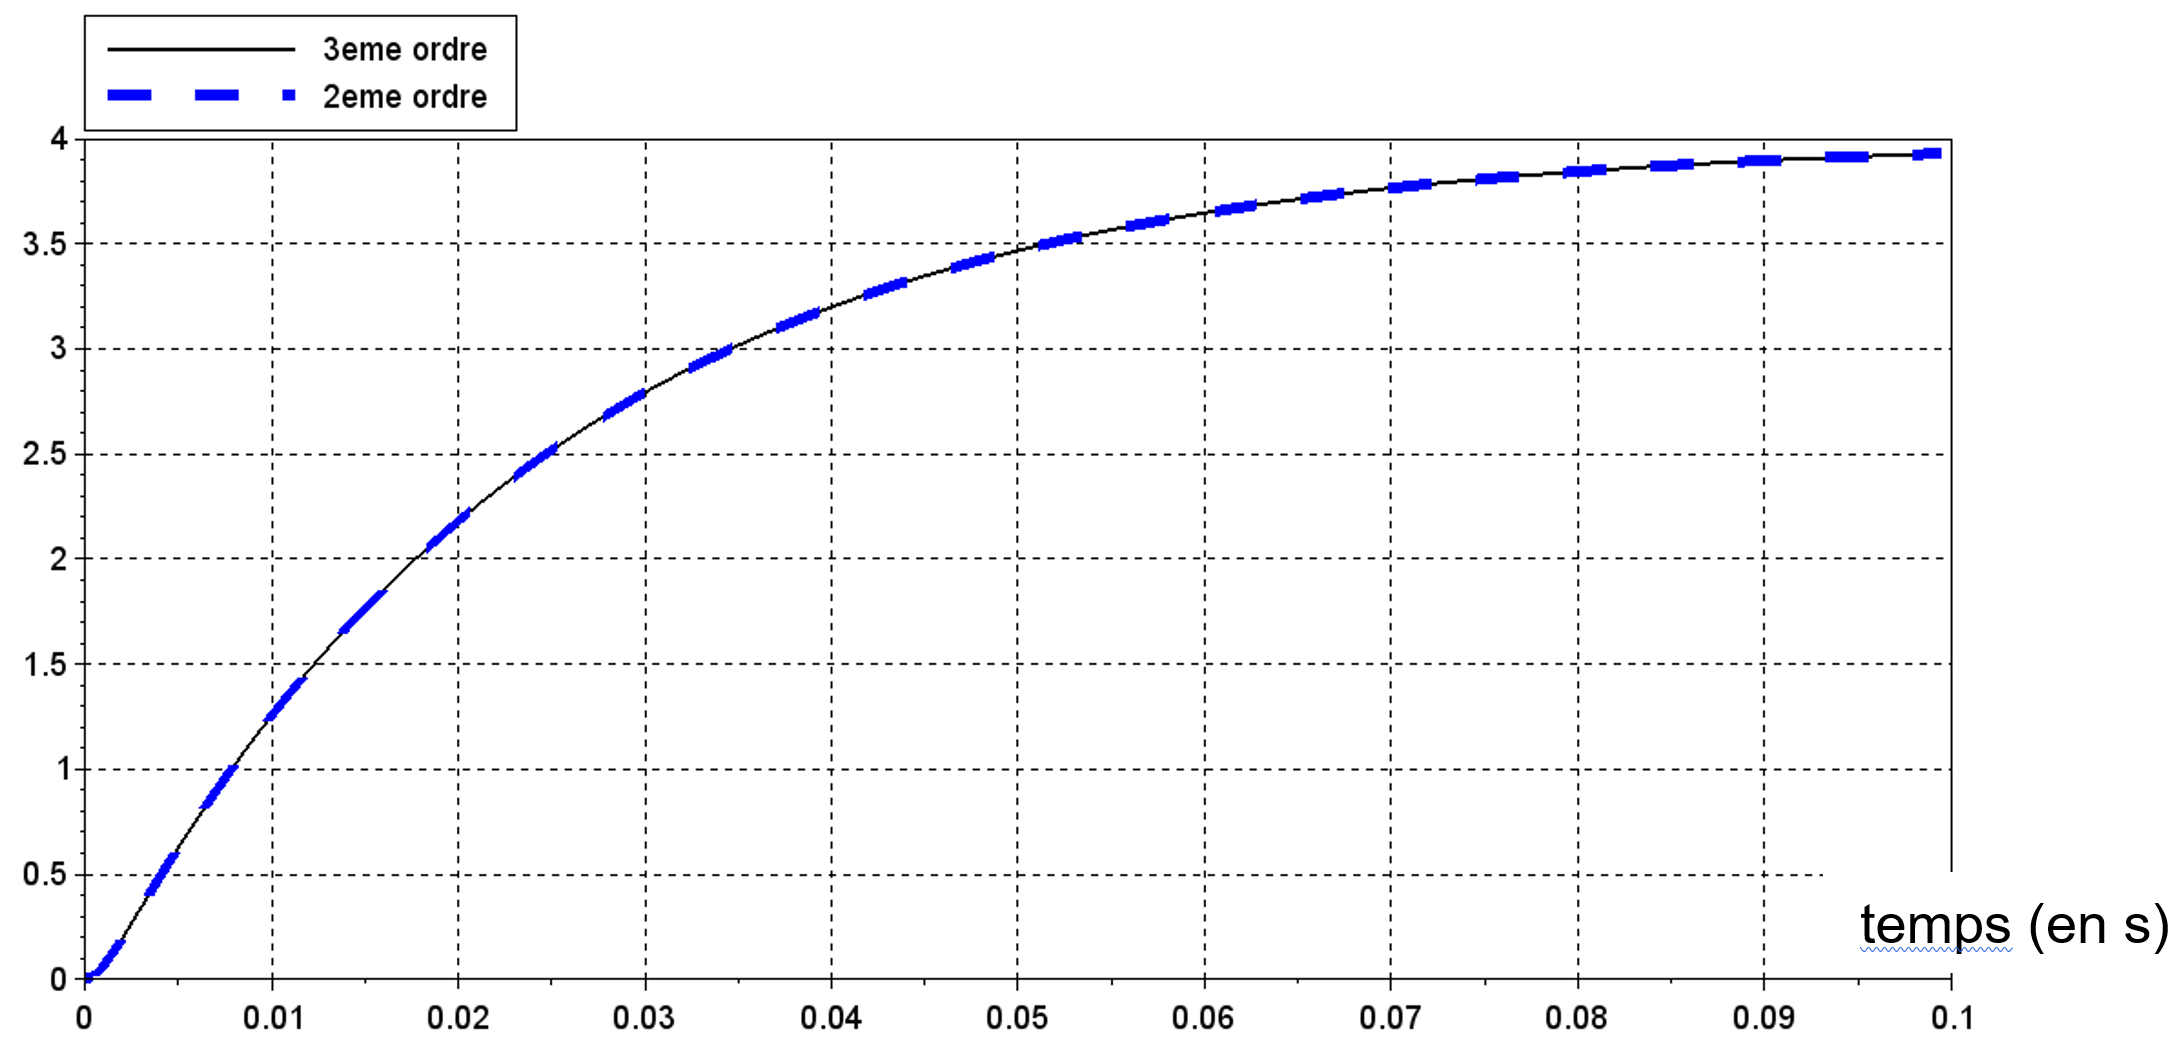
\includegraphics[width=0.8\linewidth]{img/img10}
 \caption{Influence du 3\up{ème} ordre : déplacement de la patte de dérailleur (mm) en fonction du temps (s)}
 \label{img10}
\end{figure}

On remarque sur la figure 9 que le système du 3\up{ème} ordre peut être simplifié en 2\up{ème} ordre. 

On considère que le temps mis par le système pour passer une vitesse correspond au temps mis par le système pour que le déplacement soit de 4,5 mm (4 mm de consigne plus le dépassement souhaité de 0,5 mm).

\question{En négligeant l'influence du terme de degré 3 de $H_{BF}$, déterminer son gain $K_{BF}$, $\xi$ et $\omega_0$ et faire l'application numérique ($r_0r_1r_2=0,001$ et $r_2=0,02$). Estimer à partir de l'abaque donnée en annexe le temps de réponse à 5\% mis par le système pour changer une vitesse. Déterminer si le dépassement respecte le cahier des charges.}

On souhaite maintenant régler le système, à l'aide du correcteur C(p), afin d'avoir le dépassement attendu dans le cahier des charges.

On a toujours un correcteur proportionnel $C(p)=K_{cor}$.

\question{Déterminer la valeur de $\xi$ permettant d'atteindre le dépassement maximum. En déduire la valeur $K_{cor}$ qui permet de l'obtenir. Vérifier si le temps de réponse respecte alors le cahier des charges.}

On prendra: $ln(0,125)\approx -2$, $\pi\approx 3$ et $\sqrt{0,3}\approx 0,55$.

Le temps de réponse calculé à la réponse précédente est cependant impossible à atteindre physiquement avec le matériel employé.

\question{Évaluer la tension aux bornes du moteur à l'instant initial suite à une impulsion de commande. En déduire la modification à faire au niveau de la modélisation du moteur pour diminuer l'écart entre le modèle et le comportement réel.}

\question{Que va-t-il se passer alors ? (choisir parmi les réponses suivantes:)
\begin{itemize}
 \item le système va saturer,
 \item le système va lui même choisir une tension plus adaptée à partir de calculs complexes,
 \item le système va se détériorer.
\end{itemize}}

\section{Identification de fonctions de transfert}

\begin{figure}[!h]
 \centering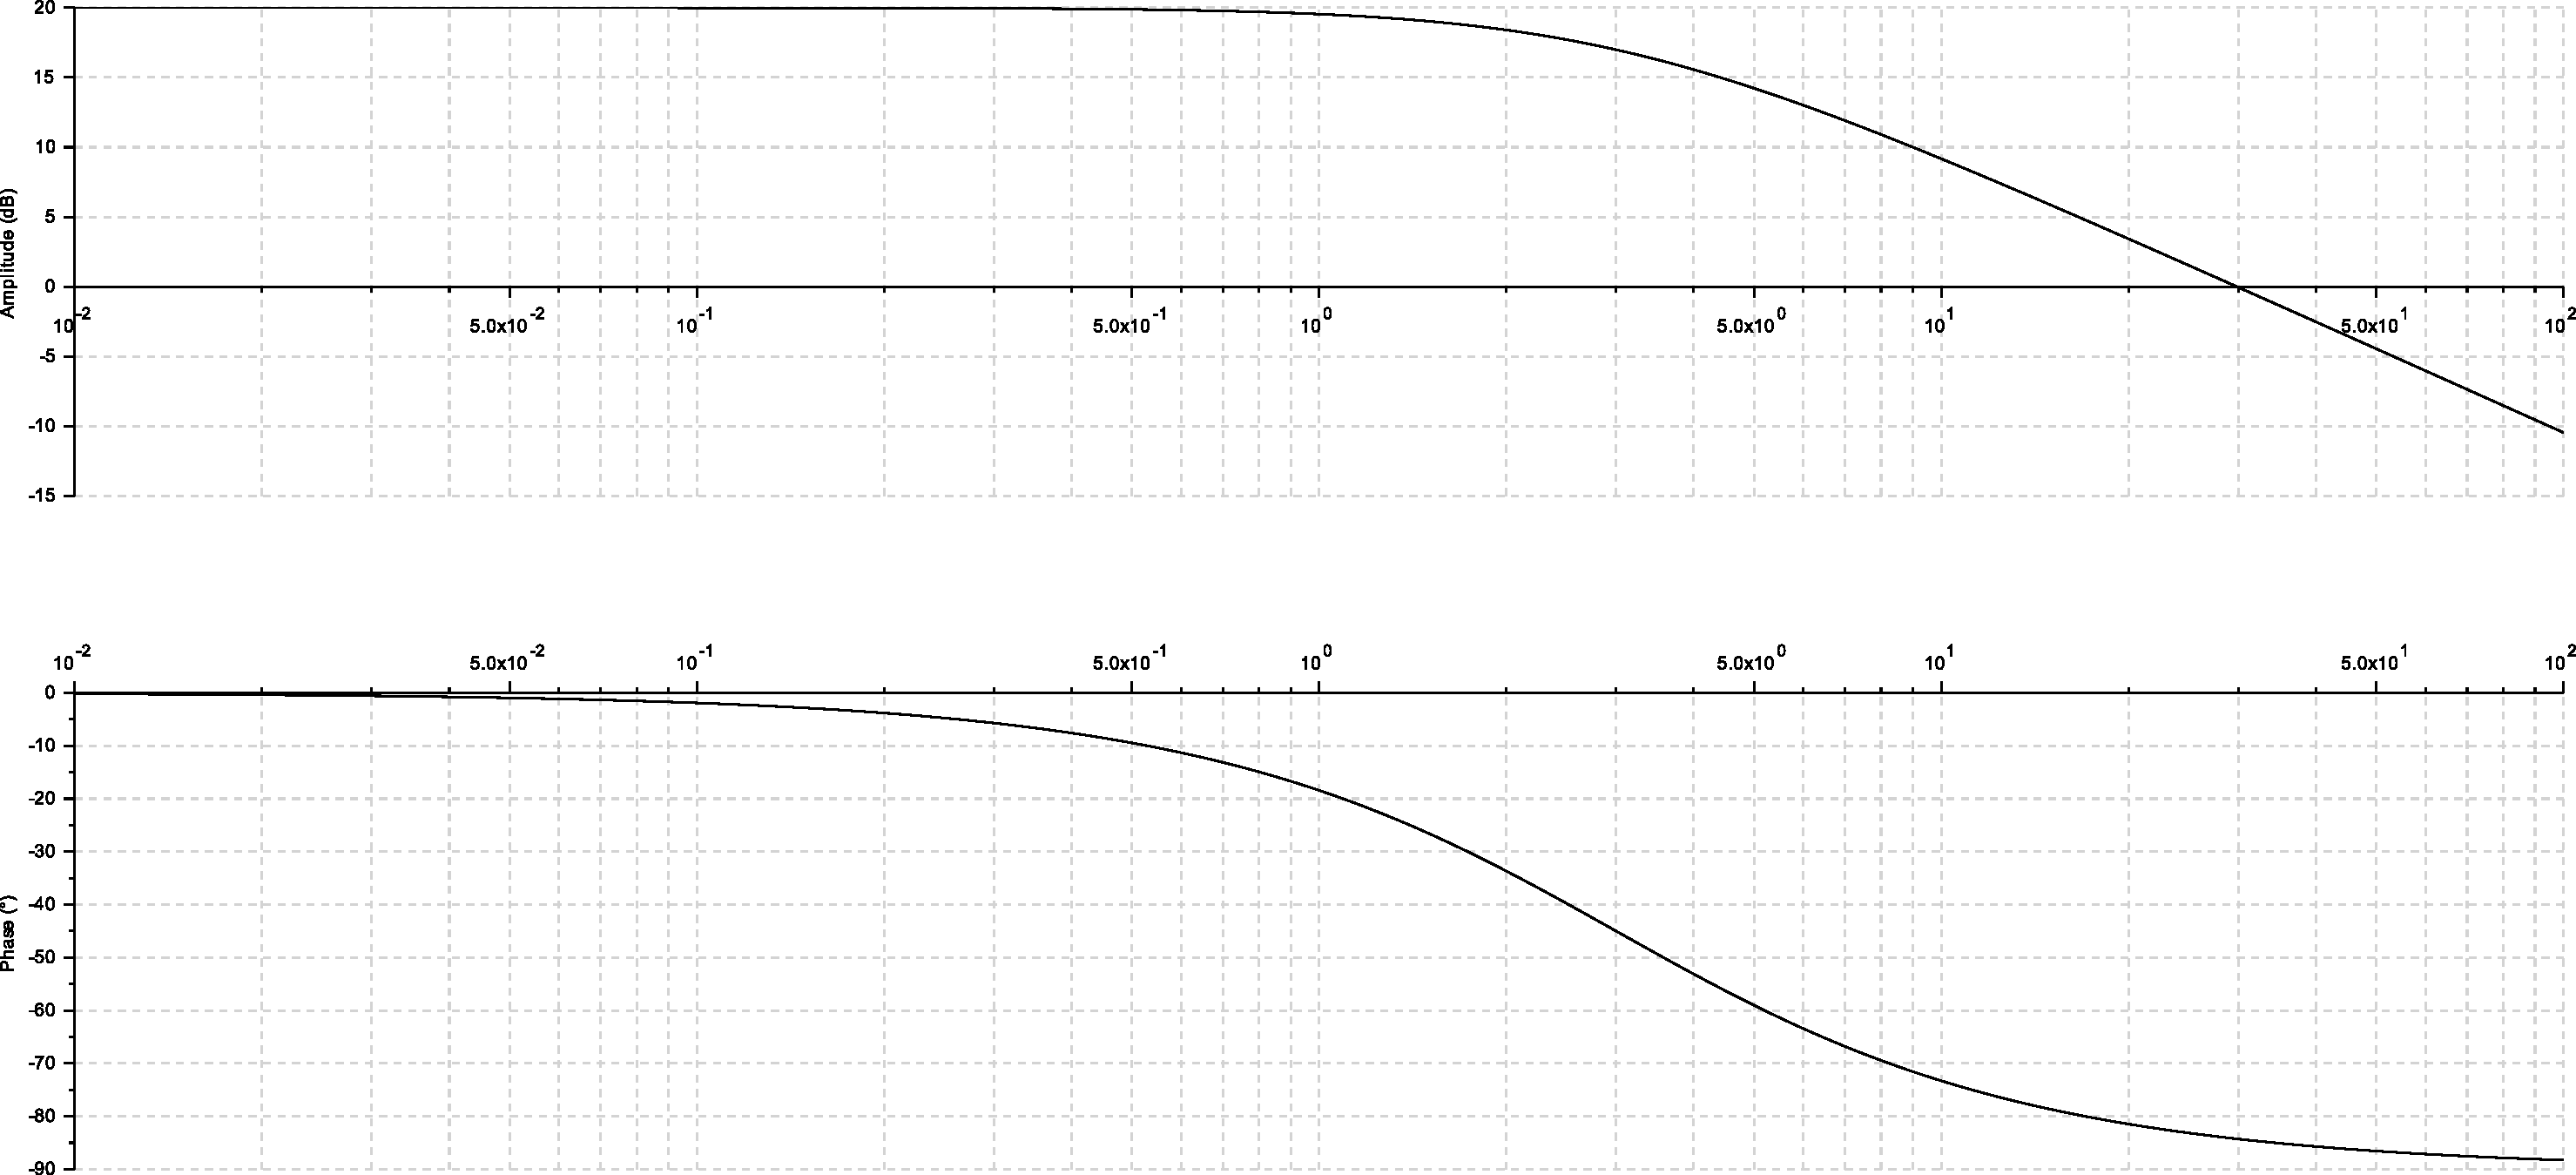
\includegraphics[width=0.8\linewidth]{img/Bode1}
 \caption{Diagrammes de Bode de la fonction de transfert $H_1(p)$.}
 \label{img11}
\end{figure}

\begin{figure}[!h]
 \centering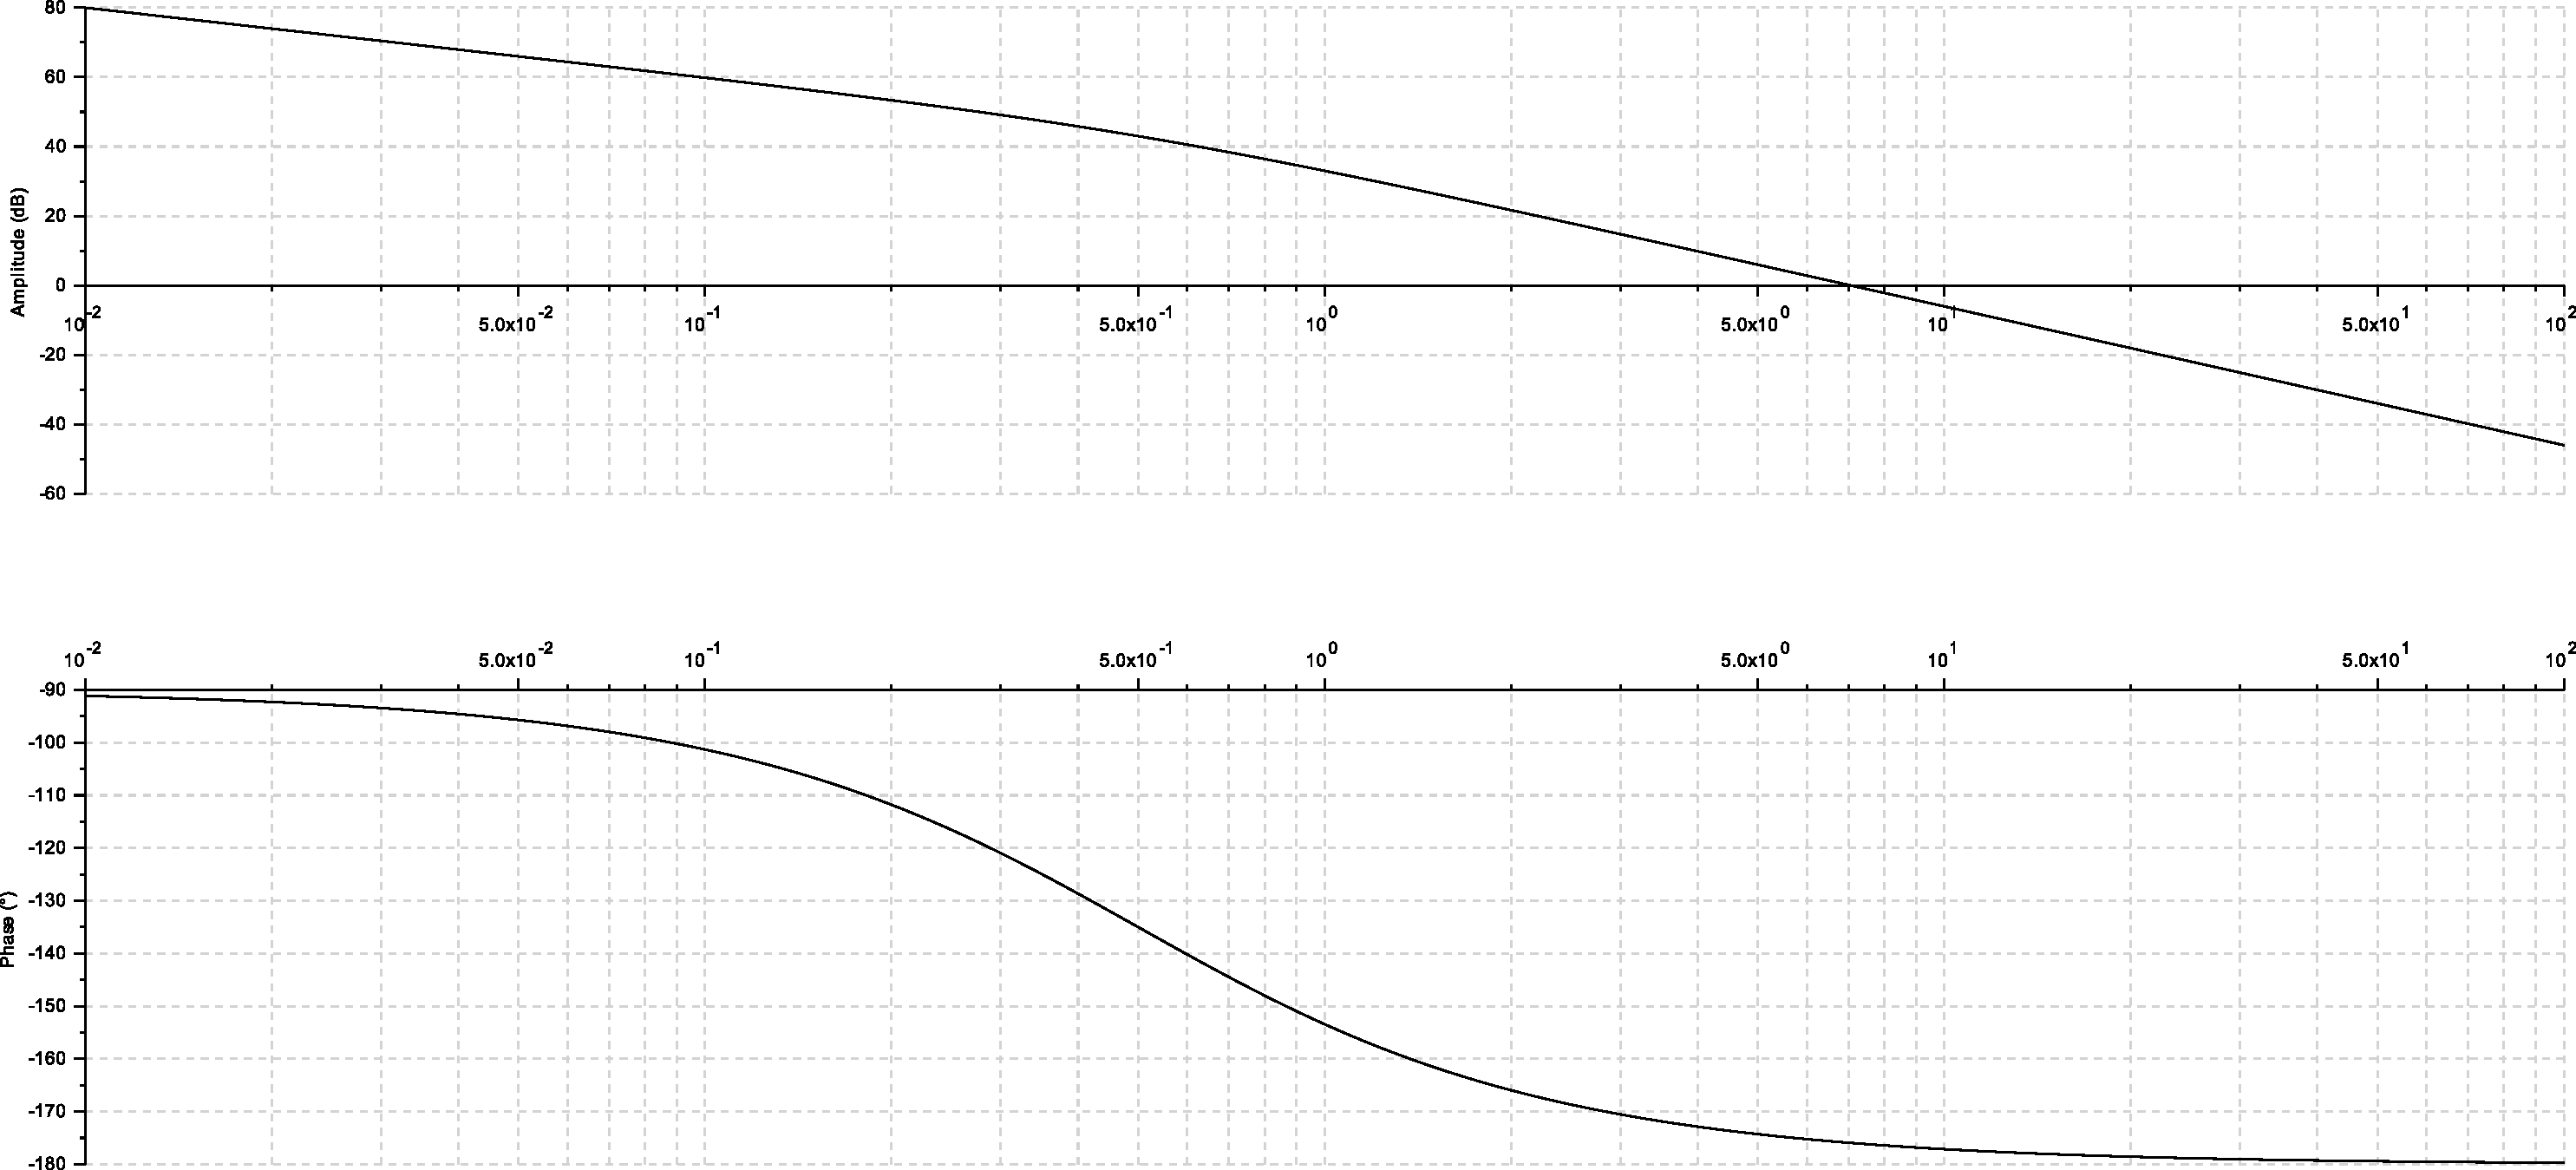
\includegraphics[width=0.8\linewidth]{img/Bode2}
 \caption{Diagrammes de Bode de la fonction de transfert $H_2(p)$.}
 \label{img12}
\end{figure}

\question{Identifier la fonction de transfert $H_1(p)$ dont les diagrammes de Bode sont présentés sur la figure \ref{img11}. L'écrire sous la forme canonique et donner la valeur de ses constantes caractéristiques.}

\question{Identifier la fonction de transfert $H_2(p)$ dont les diagrammes de Bode sont présentés sur la figure \ref{img12}. L'écrire sous la forme canonique et donner la valeur de ses constantes caractéristiques.}

\newpage

\section{Conception d'un assemblage par vis}

\begin{figure}[!h]
 \centering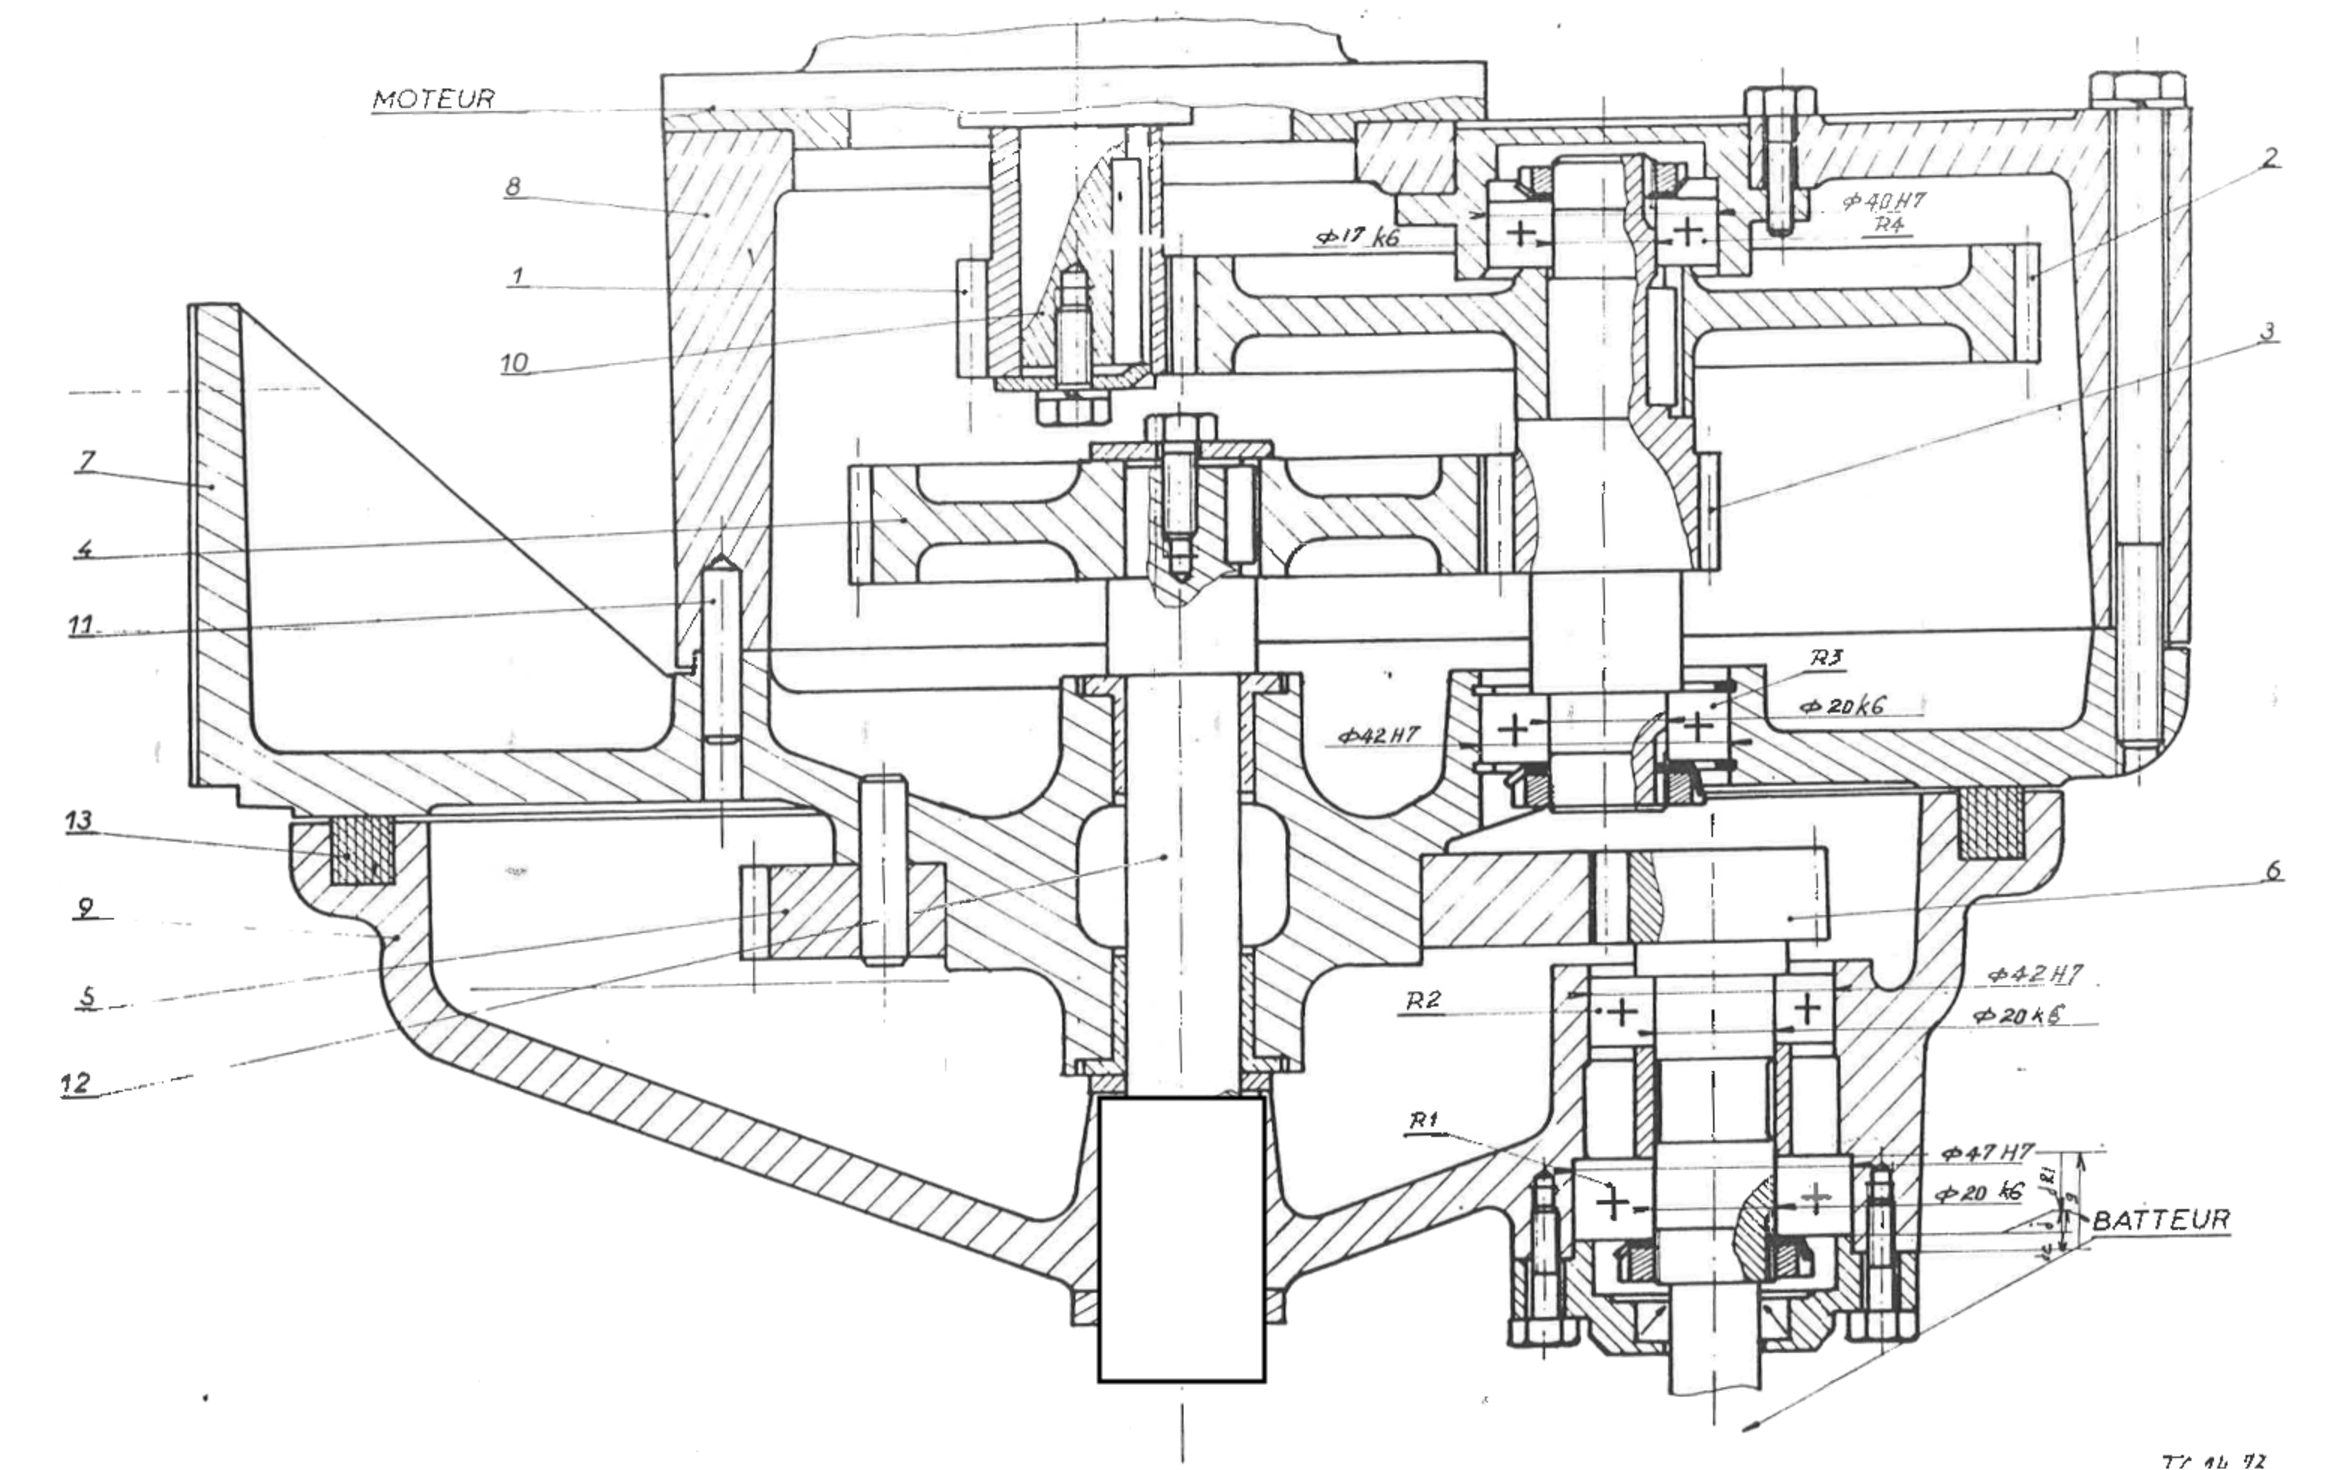
\includegraphics[width=0.9\linewidth]{img/Malaxeur_vierge}
 \caption{Conception d'un assemblage par vis}
 \label{img13}
\end{figure}

Au niveau de la zone à compléter, l'arbre 12 est cylindrique. Il est inséré dans un trou qui traverse la pièce 9. Une clavette empêche la rotation relative des deux pièces. Une vis traverse la pièce 9 et vient dans un taraudage percé dans la pièce 12. La solution demandée peut s'inspirer d'une autre zone du dessin.

\question{Compléter \textbf{le dessin du document réponse} en dessinant la solution d'assemblage vis+clavette dans le cadre prévu à cet effet.}


\cleardoublepage

\pagestyle{empty}

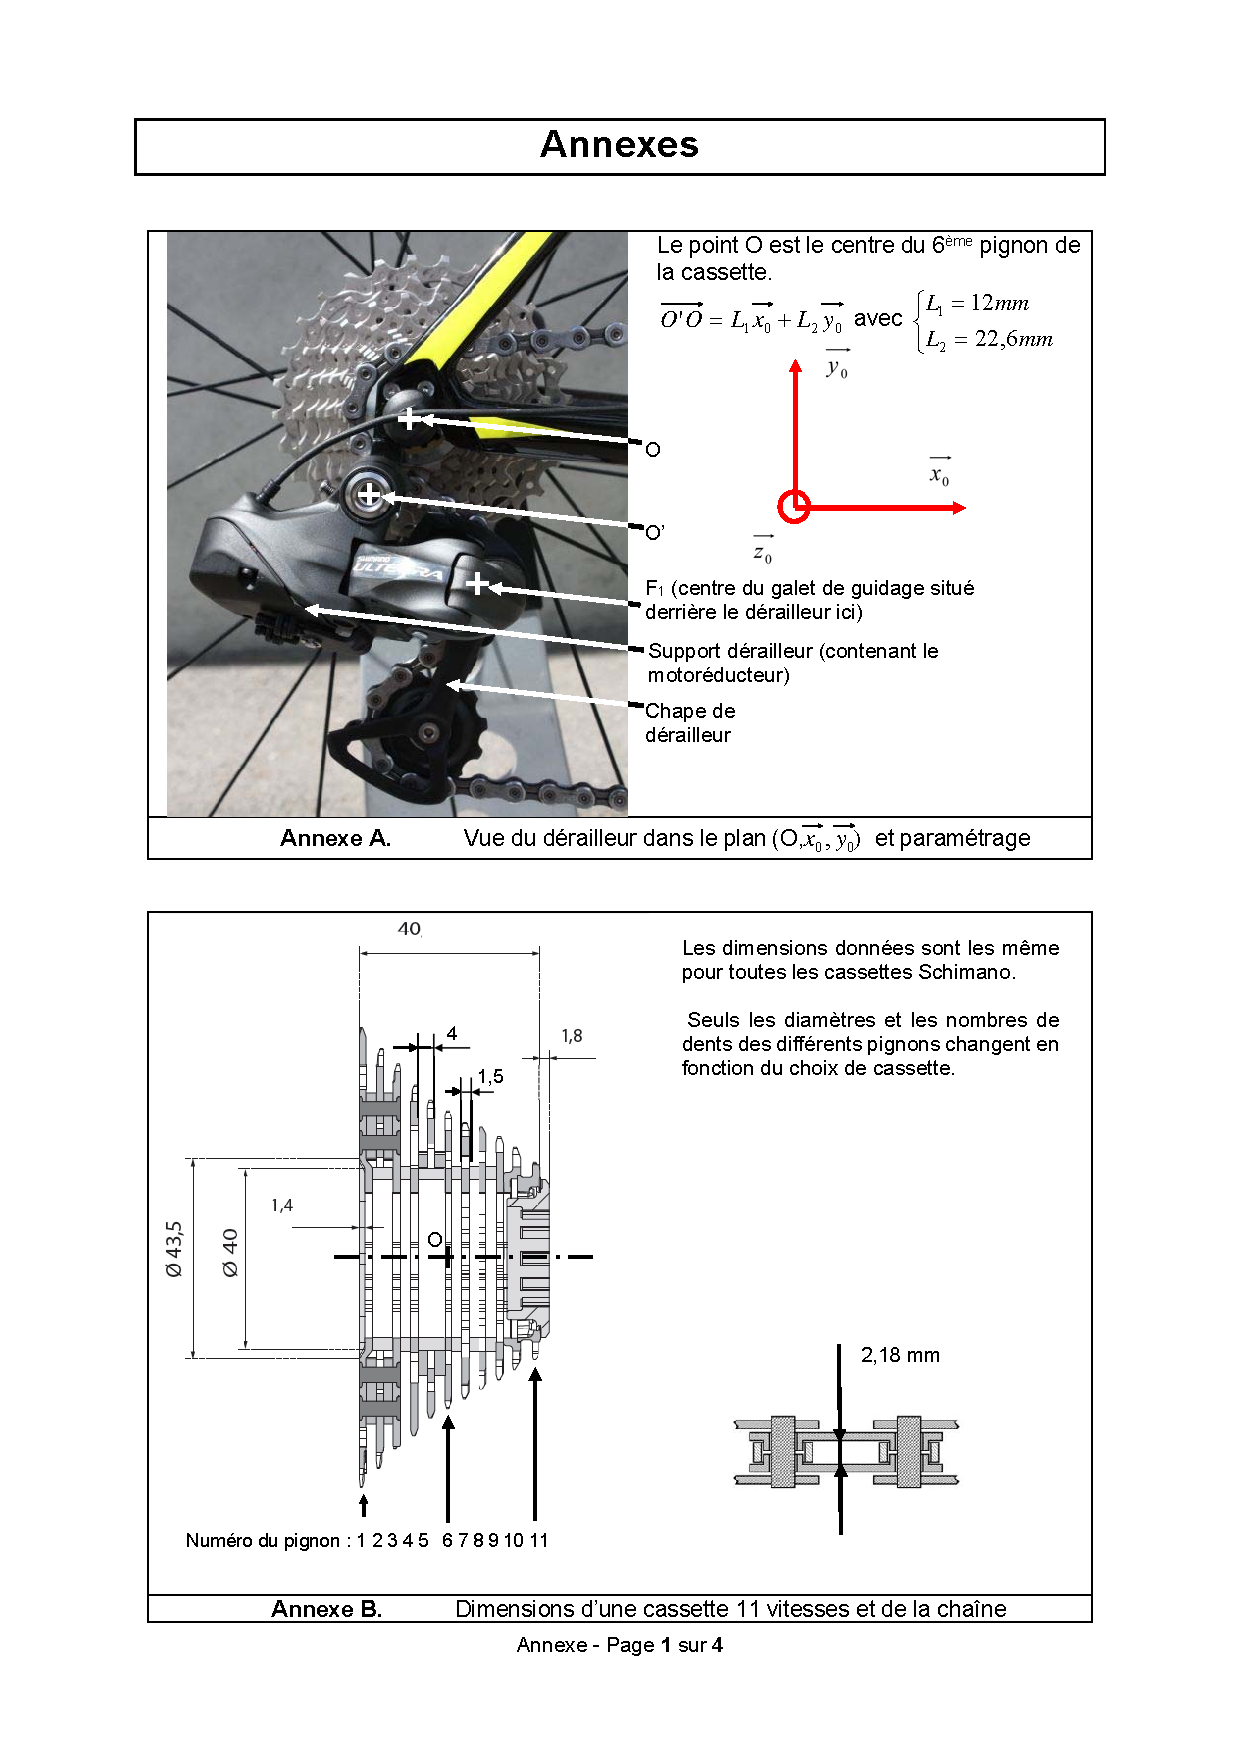
\includepdf[pages={-},scale=1,pagecommand={},offset=0cm 0cm]{img/annexes.pdf}
\newpage
\cleardoublepage

\pagestyle{documentreponse}

\section{Documents réponse}

\reponse{1}{\ifdef{\public}{\vspace{7cm}}{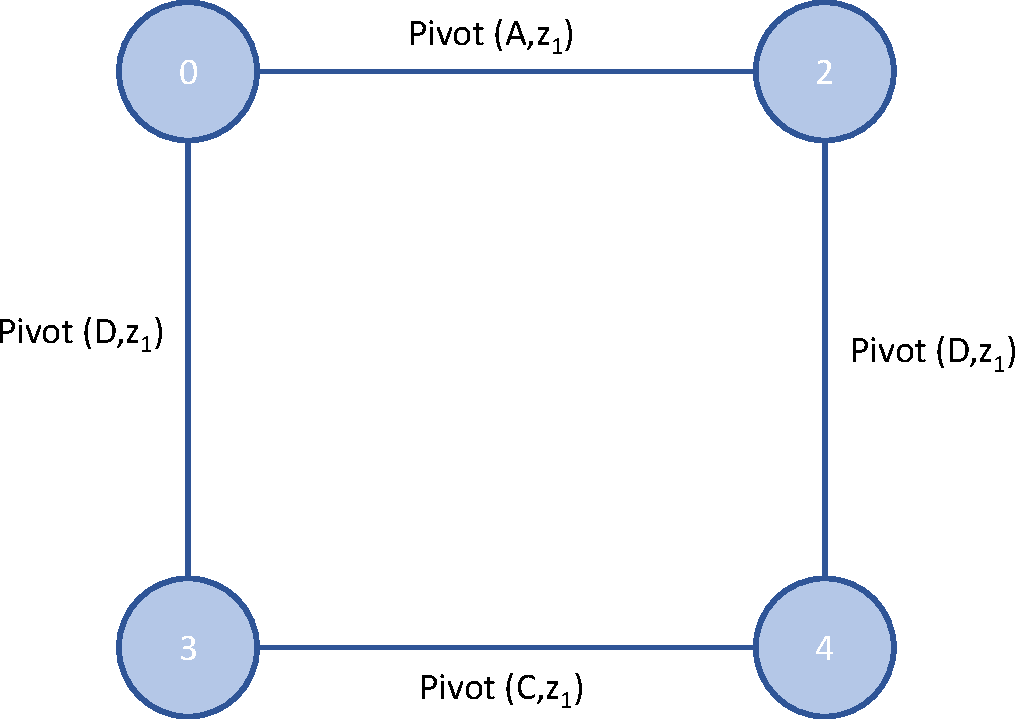
\includegraphics[width=0.5\linewidth]{img/Graphe_liaisons}}}

\reponse{1}{\ifdef{\public}{\vspace{5cm}}{
\begin{overpic}[width=0.4\textwidth]{img/Reperes}
 \put (100,5) {\textbf{$\overrightarrow{x_1}$}}
 \put (100,25) {\textbf{$\overrightarrow{x_2}$}}
 \put (7,73) {\textbf{$\overrightarrow{y_2}$}}
 \put (25,73) {\textbf{$\overrightarrow{y_1}$}}
 \put (73,6) {\textbf{$\theta$}}
 \put (-5,0) {\textbf{$\overrightarrow{z_1}=\overrightarrow{z_2}$}}
\end{overpic}\hfill
\begin{overpic}[width=0.4\textwidth]{img/Reperes}
 \put (100,5) {\textbf{$\overrightarrow{y_0}$}}
 \put (100,25) {\textbf{$\overrightarrow{y_1}$}}
 \put (7,73) {\textbf{$\overrightarrow{z_1}$}}
 \put (25,73) {\textbf{$\overrightarrow{z_0}$}}
 \put (73,6) {\textbf{$\alpha$}}
 \put (-5,0) {\textbf{$\overrightarrow{x_0}=\overrightarrow{x_1}$}}
\end{overpic}
}}

\reponse{1}{\ifdef{\public}{\vspace{1cm}}{$\overrightarrow{AB}+\overrightarrow{BC}+\overrightarrow{CD}+\overrightarrow{DA}=\overrightarrow{0}$}}

\reponse{1}{\ifdef{\public}{\vspace{4cm}}{$\left\{V_{2/0}\right\}=\left\{\begin{array}{cc}0 & 0 \\ 0 & 0 \\ \omega_{z20} & 0 \end{array}\right\}_A$, $\left\{V_{4/2}\right\}=\left\{\begin{array}{cc}0 & 0 \\ 0 & 0 \\ \omega_{z42} & 0 \end{array}\right\}_B$, $\left\{V_{4/3}\right\}=\left\{\begin{array}{cc} 0 & 0 \\ 0 & 0 \\ \omega_{z43} & 0 \end{array}\right\}_C$, $\left\{V_{3/0}\right\}=\left\{\begin{array}{cc} 0 & 0 \\ 0 & 0 \\ \omega_{z30} & 0 \end{array}\right\}_D$}}

\newpage

\reponse{1}{\ifdef{\public}{\vspace{6cm}}{$\left\{V_{2/0}\right\}=\left\{\begin{array}{cc}0 & 0 \\ 0 & 0 \\ \omega_{z20} & 0 \end{array}\right\}_A$, $\left\{V_{4/2}\right\}=\left\{\begin{array}{cc} 0 & L.sin\theta.\omega_{z42} \\ 0 & -L.cos\theta.\omega_{z42} \\ \omega_{z42} & 0 \end{array}\right\}_A$, $\left\{V_{4/3}\right\}=\left\{\begin{array}{cc} 0 & (L.sin\theta-l_1).\omega_{z43} \\ 0 & -L.cos\theta.\omega_{z43} \\ \omega_{z43} & 0 \end{array}\right\}_A$, $\left\{V_{3/0}\right\}=\left\{\begin{array}{cc} 0 & -l_1.\omega_{z30} \\ 0 & 0 \\ \omega_{z30} & 0 \end{array}\right\}_A$}}

\reponse{1}{\ifdef{\public}{\vspace{6cm}}{\begin{eqnarray}0+0=0+0 \\ 0+0=0+0 \\ \omega_{z42}+\omega_{z20}=\omega_{z43}+\omega_{z30} \\ L.sin\theta.\omega_{z42}+0=(L.sin\theta-l_1).\omega_{z43}-l_1.\omega_{z30} \\ -L.cos\theta.\omega_{z42}+0=-L.cos\theta.\omega_{z43}+0 \\ 0+0=0+0 \end{eqnarray}}}

\reponse{1}{\ifdef{\public}{\vspace{6cm}}{D'après l'équation 5, $\omega_{z42}=\omega_{z43}$, donc en utilisant ce résultat dans l'équation 4, on obtient $0=l_1.(\omega_{z43}+\omega_{z30})$, donc $\omega_{z43}+\omega_{z30}=\omega_{z40}=0$, donc $\|\overrightarrow{\Omega_{4/0}}\|=0$, cela signifie que l'orientation de la droite (BC) ne change pas, elle est toujours verticale.}}

\newpage

\reponse{1}{\ifdef{\public}{\vspace{4cm}}{$\overrightarrow{AB}=L.cos\theta.\overrightarrow{x_1}+L.sin\theta.\overrightarrow{y_1}$.}}

\reponse{1}{\ifdef{\public}{\vspace{4cm}}{$\overrightarrow{AB_1}=L.cos(-60).\overrightarrow{x_1}+L.sin(-60).\overrightarrow{y_1}$, $\overrightarrow{AB_2}=L.cos60.\overrightarrow{x_1}+L.sin60.\overrightarrow{y_1}$, donc $\overrightarrow{B_1B_2}=2.L.sin60.\overrightarrow{y_1}$}}

\reponse{1}{\ifdef{\public}{\vspace{4cm}}{$d=\overrightarrow{AB}.\overrightarrow{z_0}=L.sin\theta.sin\alpha$}}

\reponse{1}{\ifdef{\public}{\vspace{4cm}}{Le défaut de positionnement max est $\frac{2,18-1,5}{2}=0,34mm$.}}

\newpage

\reponse{1}{\ifdef{\public}{\begin{figure}[!h]
 \centering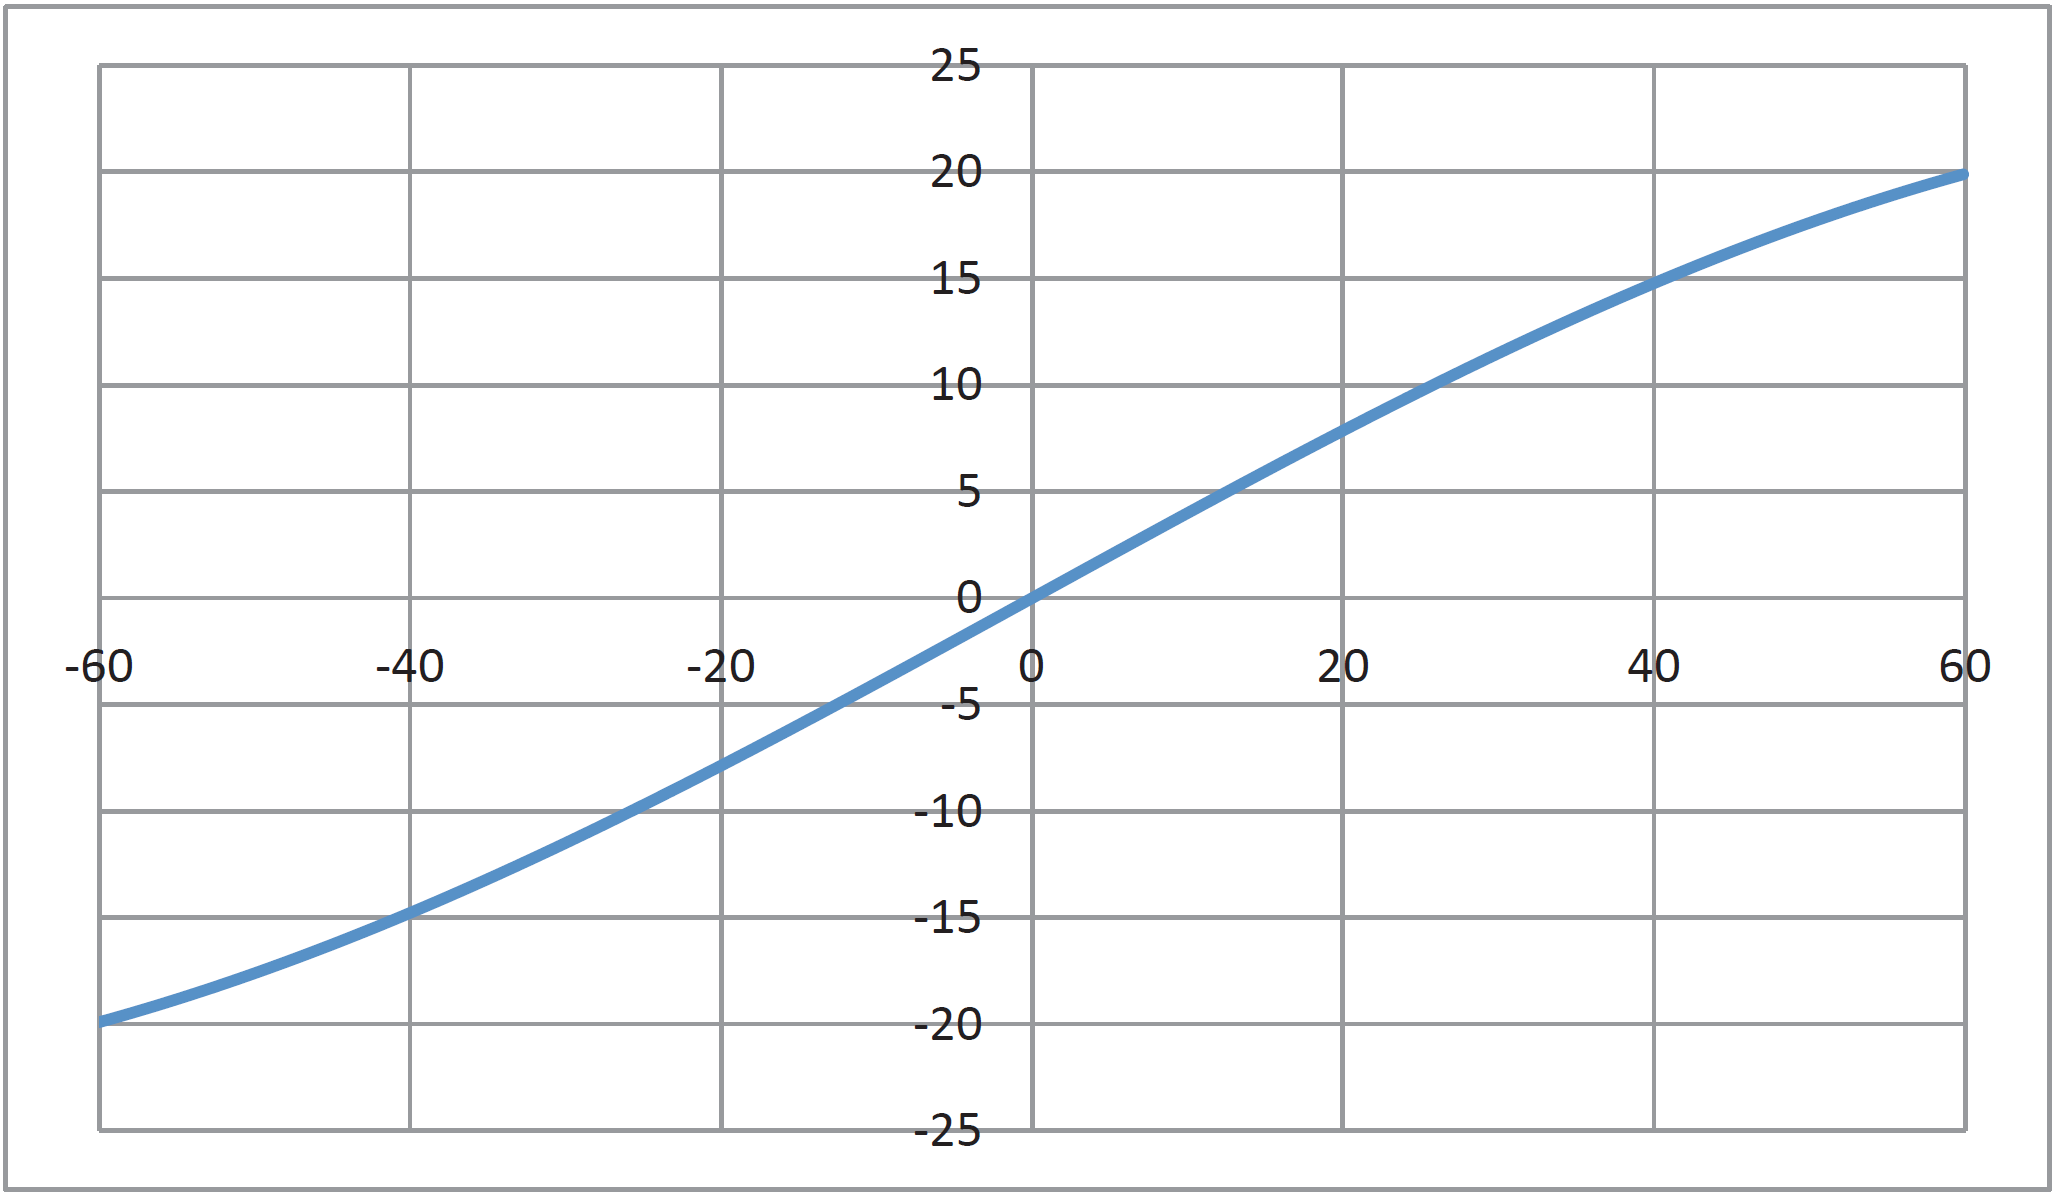
\includegraphics[width=0.8\linewidth]{img/DR1}
 \caption{$d(\theta)$ en mm en fonction de $\theta$ en degré.}
 \label{dr1}
\end{figure}}{\begin{figure}[!h]
 \centering\includegraphics[width=0.8\linewidth]{img/DR1_C}
 \caption{$d(\theta)$ en mm en fonction de $\theta$ en degré.}
 \label{dr1c}
\end{figure}}}

\reponse{1}{\ifdef{\public}{\vspace{4cm}}{L'erreur maximale entre la droite $y=3,5.x$ et la courbe est de 1 mm. L'écart entre l'intérieur de la chaine et la largeur d'un pignon est de 0,34 mm. L'erreur n'est pas admissible.}}

\reponse{1}{\ifdef{\public}{\vspace{4cm}}{$e(Z_{F_1})=\sqrt{X_{F_1}^2+Y_{F_1}^2}-R_{galet}-R_{pignon}(Z_{F_1})$, la forme d'escalier vient de $R_{pignon}(Z_{F_1})$.}}

\newpage

\reponse{1}{\ifdef{\public}{\vspace{4cm}}{La distance entre les pignons est toujours positive donc il est possible de changer les vitesses.}}

\reponse{1}{\ifdef{\public}{\vspace{4cm}}{La plus petite distance entre les pignons est au niveau du plus grand pignon, c'est donc là qu'il faut faire le réglage.}}

\reponse{1}{\ifdef{\public}{\vspace{4cm}}{D'après les équations du moteur, on a déjà montré que $\frac{\Omega(p)}{U(p)}=\frac{K}{K^2+J.P.(R+L.p)}$, de plus $\theta_m(p)=\frac{1}{p}.\Omega_m(p)$, donc $H(p)=\frac{K}{p.(K^2+J.P.(R+L.p))}$}}

\reponse{1}{\ifdef{\public}{\vspace{4cm}}{Le bloc \og 4 \fg vient des 4 mm qui séparent chaque pignon, en effet, une impulsion décale d'un pignon par rapport au pignon de départ, cela correspond à un décalage de 4 mm. $d_{cons}$ est donc lui aussi en mm.}}

\newpage

\reponse{1}{\ifdef{\public}{\vspace{4cm}}{$N_{fr\_mes}=\frac{4.n.\theta_1}{2.\pi}$, donc $B=\frac{4.n}{2.\pi}$.}}

\reponse{1}{\ifdef{\public}{\vspace{4cm}}{$B=4,4$, $A=\frac{B}{20,05*r_2}\approx11mm^{-1}$.}}

\reponse{1}{\ifdef{\public}{\vspace{4cm}}{$H_{BF}=\frac{\frac{80,2.A.r_2}{B}}{1+\frac{p}{K.B.r_0.r_1}.(K^2+J.p.(R+L.p))}$}}

\reponse{1}{\ifdef{\public}{\vspace{4cm}}{$K_{BF}=\frac{80,2.A.r_2}{B}\approx4mm$, $\xi=\frac{K}{2}.\sqrt{\frac{K}{J.R.B.r_0.r_1.K_{cor}}}=2,8$ et  $\omega_0=\sqrt{\frac{K.B.r_0.r_1.K_{cor}}{J.R}}\approx220rad.s^{-1}$. Ainsi, on lit sur l'abaque $\omega_0.t_{R5\%}=16$, donc $t_{R5\%}=0,08s$.}}

\newpage

\reponse{1}{\ifdef{\public}{\vspace{4cm}}{Un dépassement de 0,5 correspond à 12,5\%. Donc $\xi=\sqrt{\frac{ln^2(0,125)}{\pi^2+ln^2(0,125)}}=0,55$ donc $K_{cor}=\left(\frac{2,8}{0,55}\right)\approx 25V/front$, cela donne un temps de réponse $t_{R5\%}=45ms$ ce qui respecte le cahier des charges.}}

\reponse{1}{\ifdef{\public}{\vspace{4cm}}{$U_{mot}=4.A.K_{cor}=1120V$}}

\reponse{1}{\ifdef{\public}{\vspace{4cm}}{Le moteur va saturer.}}

\reponse{1}{\ifdef{\public}{\vspace{2cm}}{$H_1(p)=\frac{10}{1+\frac{p}{3}}$}}

\reponse{1}{\ifdef{\public}{\vspace{2cm}}{$H_1(p)=\frac{100}{p.(1+2.p)}$}}

\newpage

\reponse{1}{\ifdef{\public}{\begin{center}
	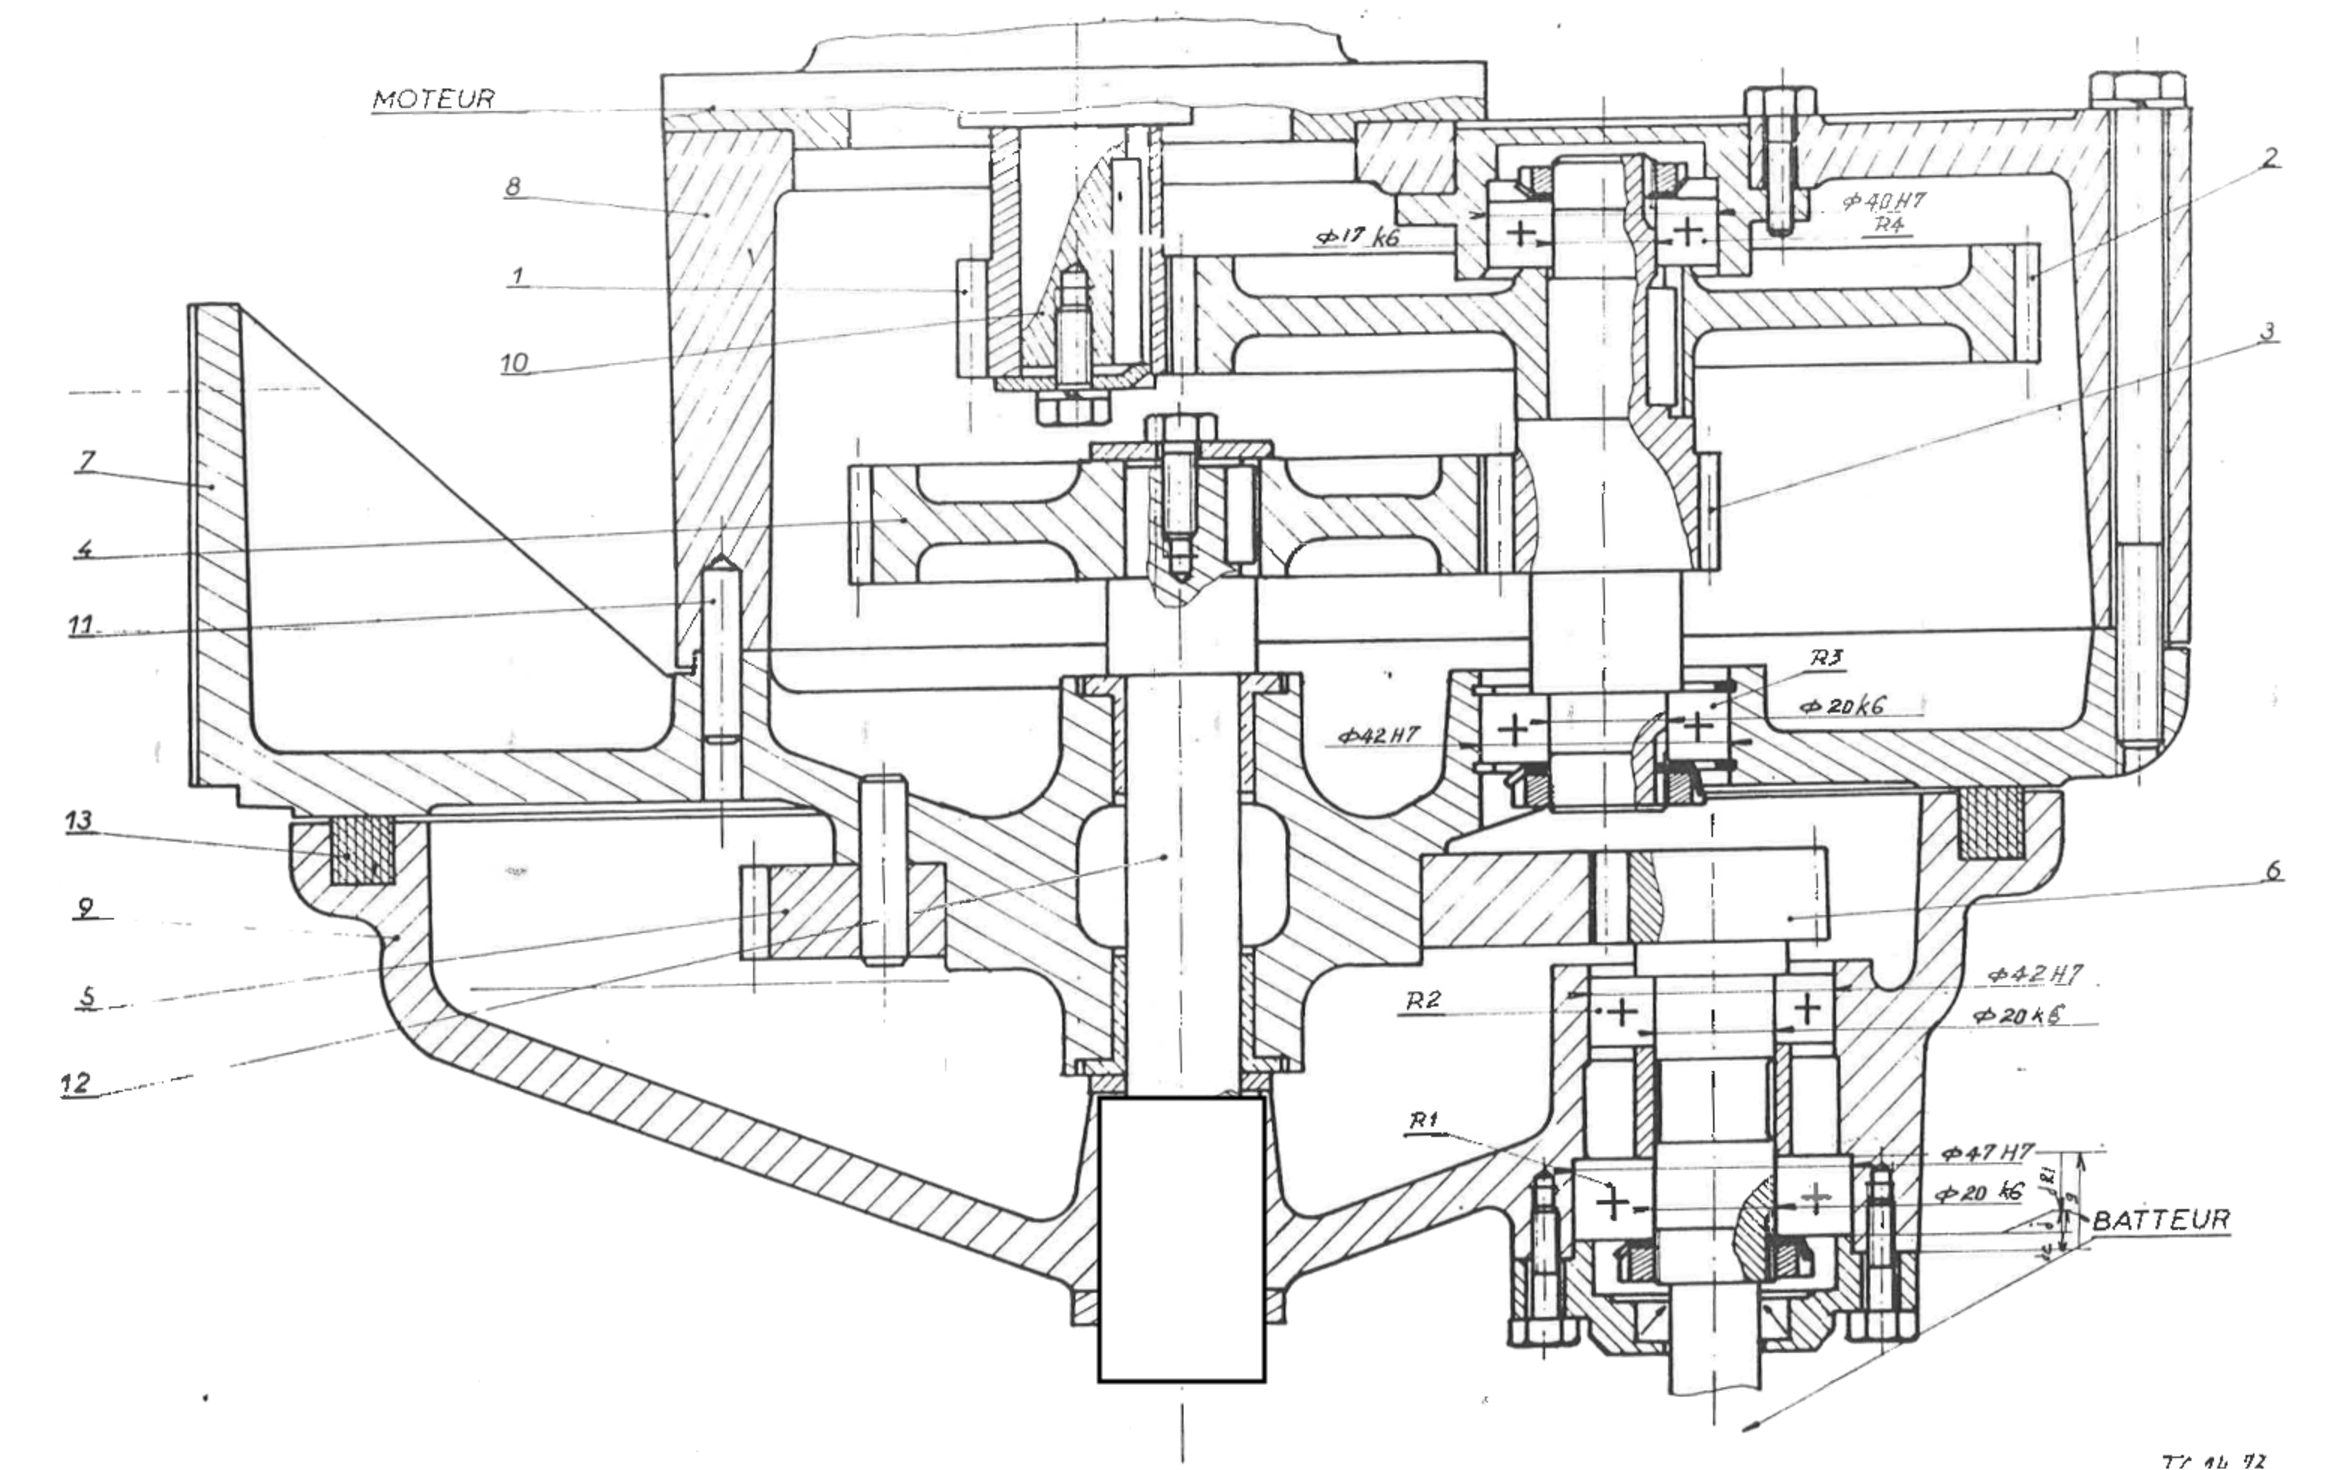
\includegraphics[width=0.9\linewidth]{img/Malaxeur_vierge}
\end{center}}{\begin{center}
	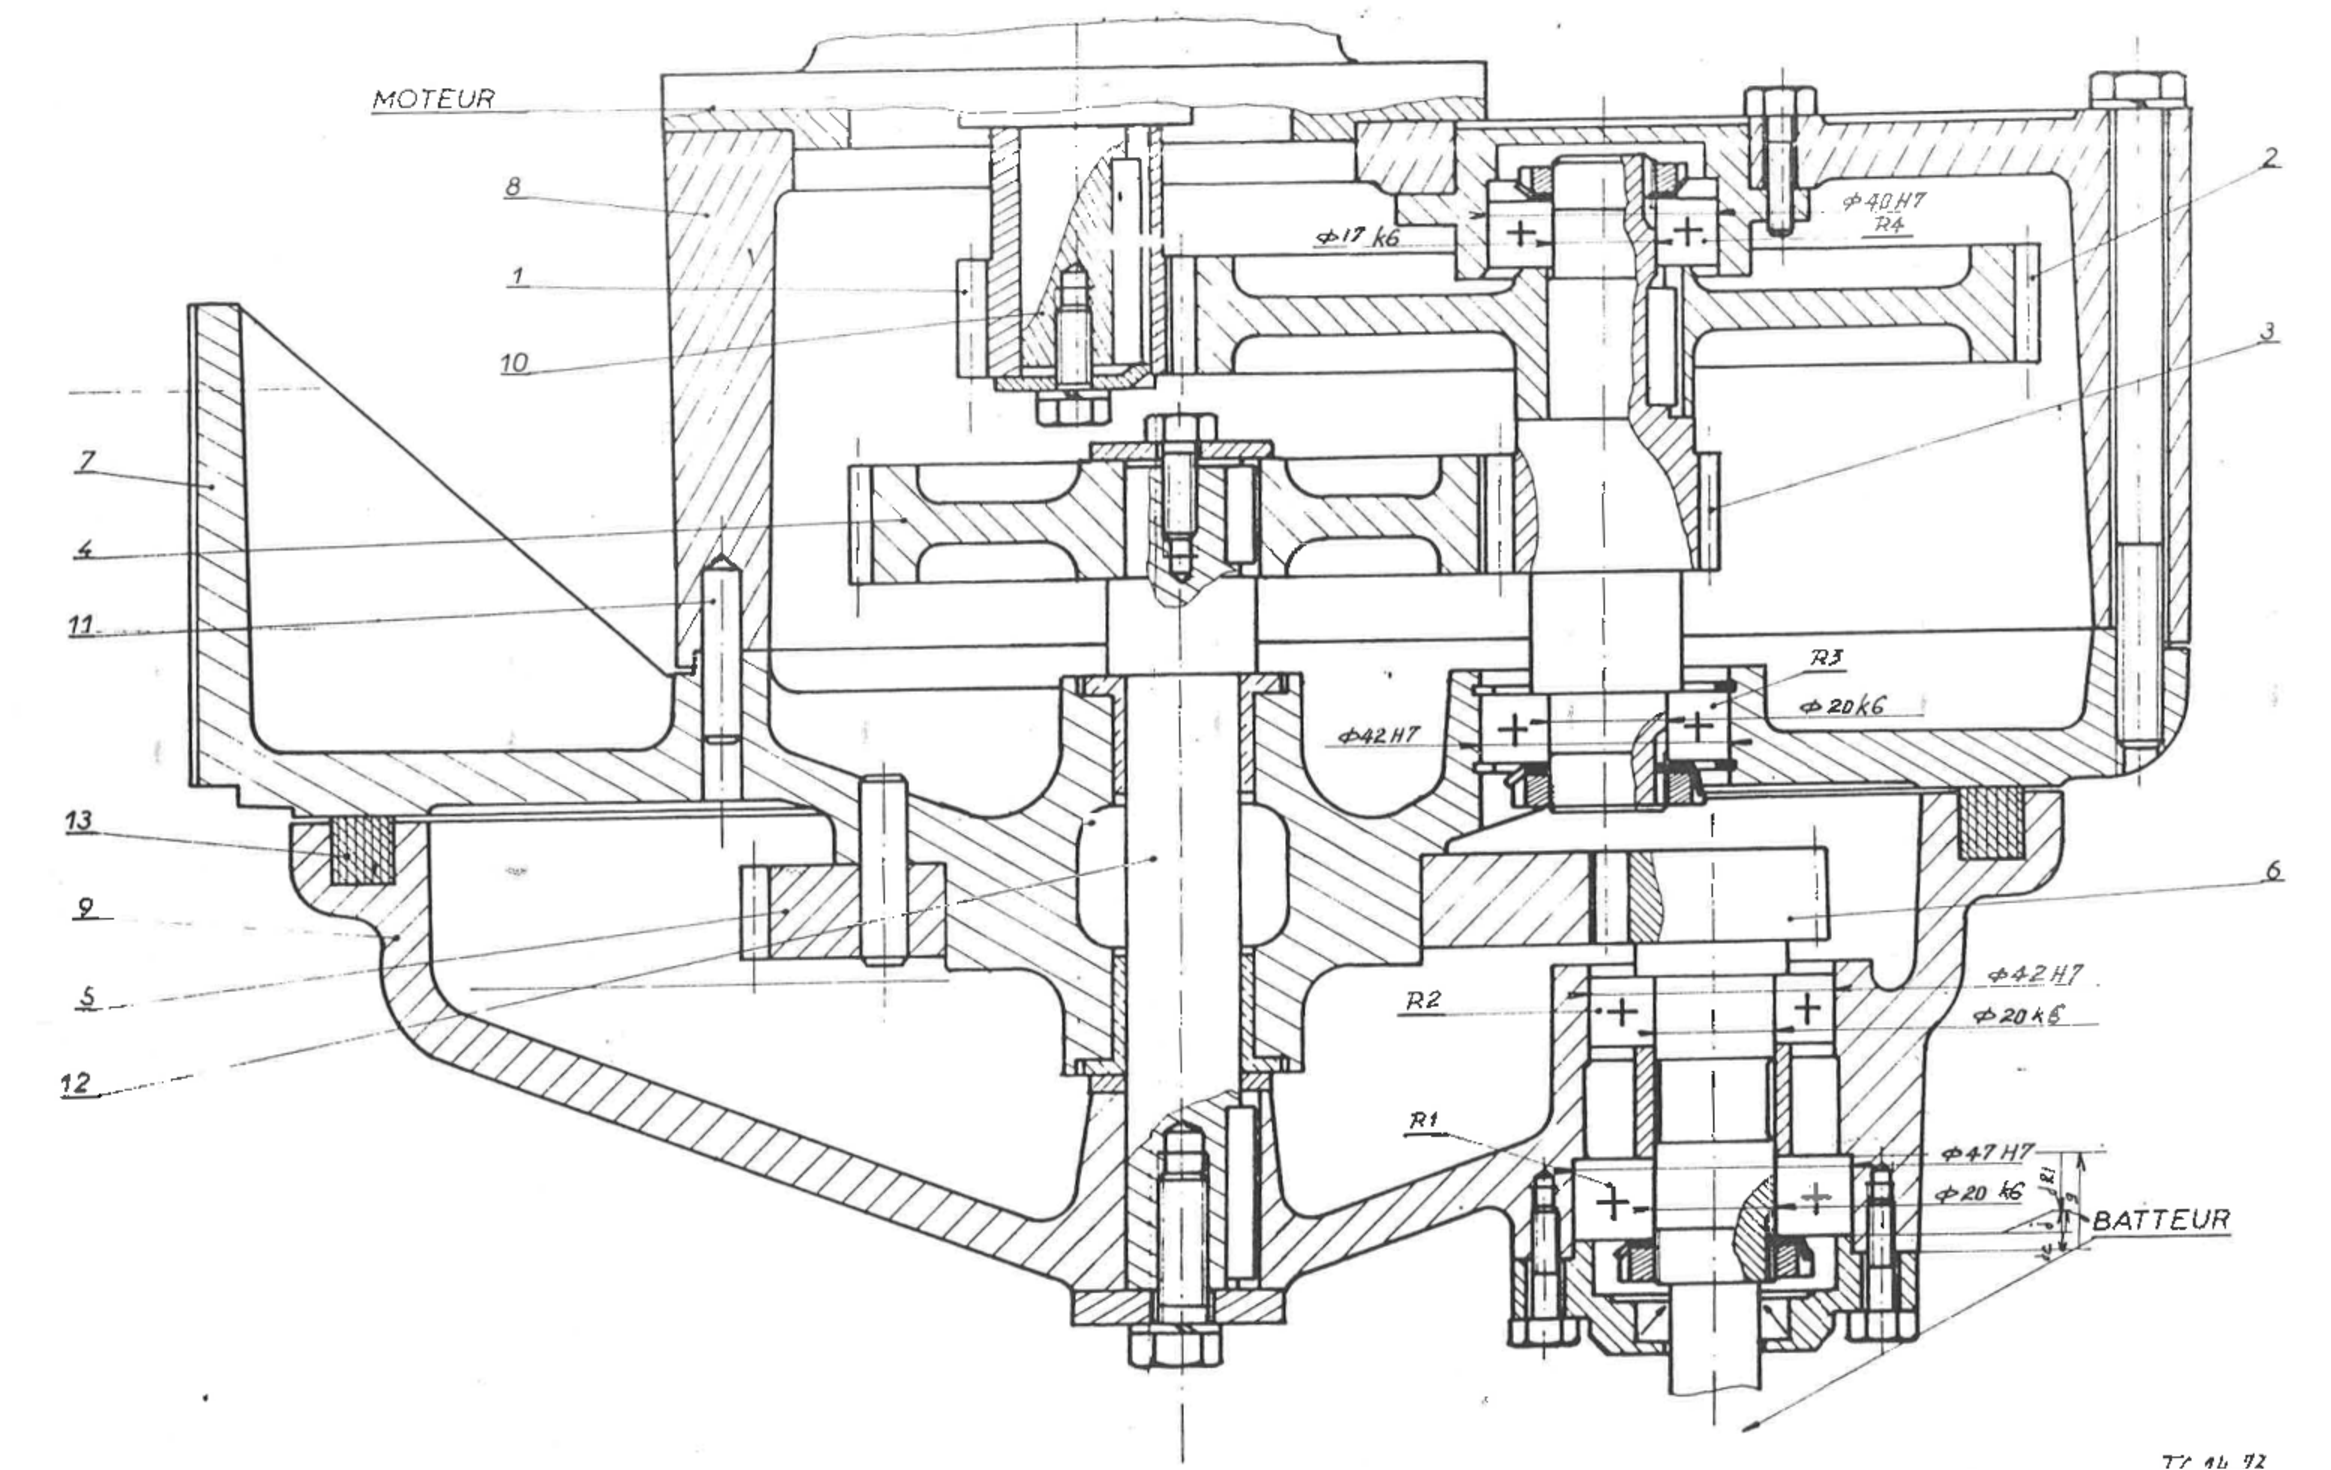
\includegraphics[width=0.9\linewidth]{img/Malaxeur}
\end{center}}}



\end{document}

